\clearpage
\section{Devices fabrication and cryogenic measurement setup}

In this section, we will discuss the fabrication and installation of our devices and the circuit setup for the measurement. The overall process in our experiment is firstly fabrication, and then inspect the chip under the microscope and probably SEM, depending on which steps we are in. After that, we bond the chip on the daughter board and load the sample into the measurement and readout circuit in the 4K board station or dilution fridge. We use QCoDes and Labber to collect data and then analyze it in Python. All fabrications were done in the Center of Quantum Device, University of Copenhagen.

\subsection{Qubit island design and simulation}
\subsubsection{Floating design}
\begin{figure}[h!]
    \centering
    \begin{subfigure}[b]{0.8\textwidth}
         \centering
         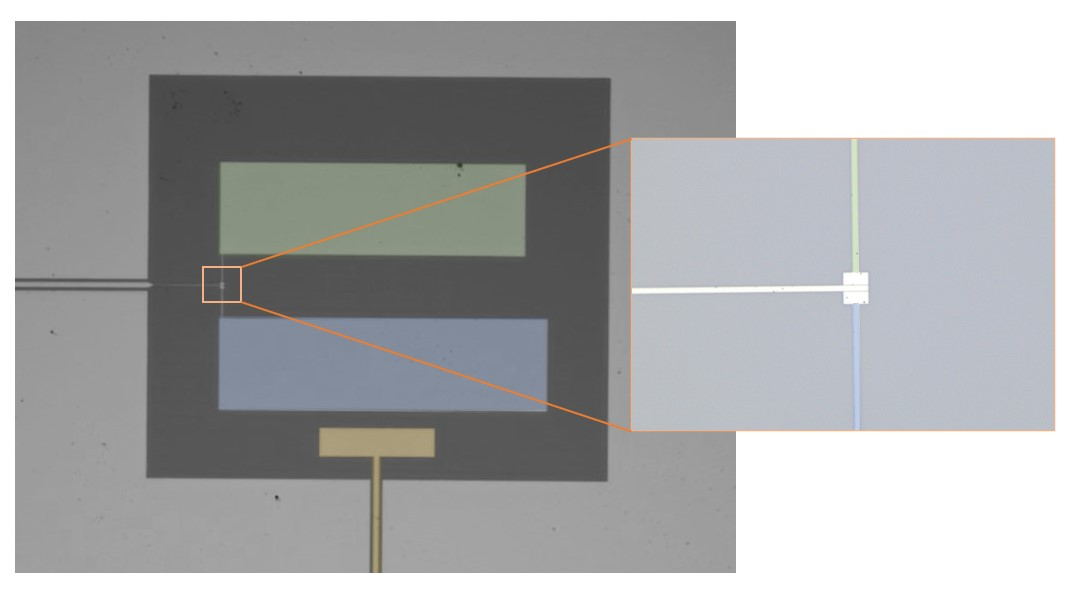
\includegraphics[width=\textwidth]{Pic/FalsecolorDesign.jpg}
         \caption{}
         \label{floatingtransmon_real}
     \end{subfigure}
     \hfill
     \begin{subfigure}[b]{0.5\textwidth}
         \centering
         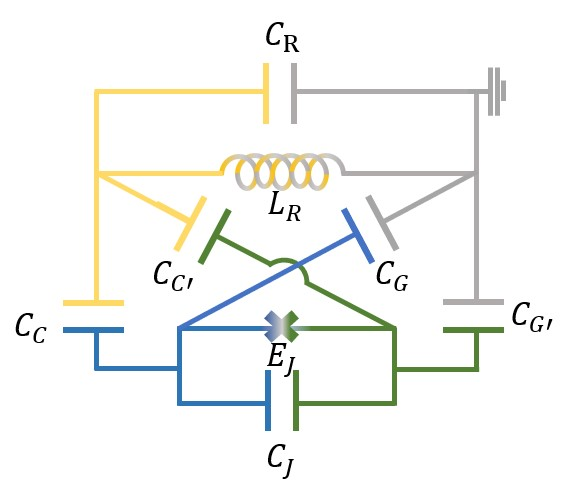
\includegraphics[width=\textwidth]{Pic/Floating transmon circuit.jpg}
         \caption{}
         \label{floatingtransmon_circuit}
     \end{subfigure}
    \caption{(\textbf{a}): False color overall floating design of the nanowire-based gatemon, the yellow pad with a downward line is connected to the resonator, and the left no color line is the electric field gate connected to a voltage source. The surrounding metal substrate is connected to the ground. (\textbf{b}): Equivalent circuit without the gate.}
    \label{floatingtransmon}
\end{figure}
Our initial design is from A.Gyenis, similar to the floating design transmon circuit (Fig.\ref{floatingtransmon}). The equivalent circuit can be drawn as Fig.\ref{floatingtransmon}(b). The total capacitance in the charging energy term is:
\begin{equation}
    C_{\phi} = C_J + \frac{(C_{C}+C_{G})(C_{C'}+C_{G'})}{C_{C}+C_{C'}+C_{G}+C_{G'}}
\end{equation}
and coupling capacitance:
\begin{equation}
    C_{coup} = \frac{C_{G'}C_{C}-C_{C'}C_{G}}{C_{C}+C_{C'}+C_{G}+C_{G'}}
\end{equation}
Then we can calculate (All the units in energy is GHz and capacitance in fF):
\begin{equation}
    \begin{array}{cc}
    E_C =& 19.37 / C_\phi \\
    \beta =& |\frac{C_\phi}{C_{coup}}| \\
    g =& 0.125\cdot\beta f_R (E_J/32E_C)^{\frac{1}{4}} \\
    \hbar\omega_{01} =& \sqrt{8E_CE_J} - E_C
    \end{array}
\end{equation}
where $f_R$ is the resonator frequency that is can be simulated in HFSS and measured through VNA. $E_J$ is the Josephson energy calculated from Ambegaokar-Baratoff relation\cite{RN39}:
\begin{equation}
    I_CR_N = \frac{\pi\Delta}{2e}
\end{equation}
and Eq.\ref{JJenergy}. The critical current can be tuned by the gate, and the normal resistance in our SNS junctions varies significantly, ranging from 4-30k$\Omega$ before exponentially resistance increase to pinch off. All the capacitance components can be calculated through Ansys Maxwell 3D.

To understand how the gate affects the nanowire, we also simulate the electric field in the design by Maxwell 3D under the distribution. 

\begin{figure}
    \centering
    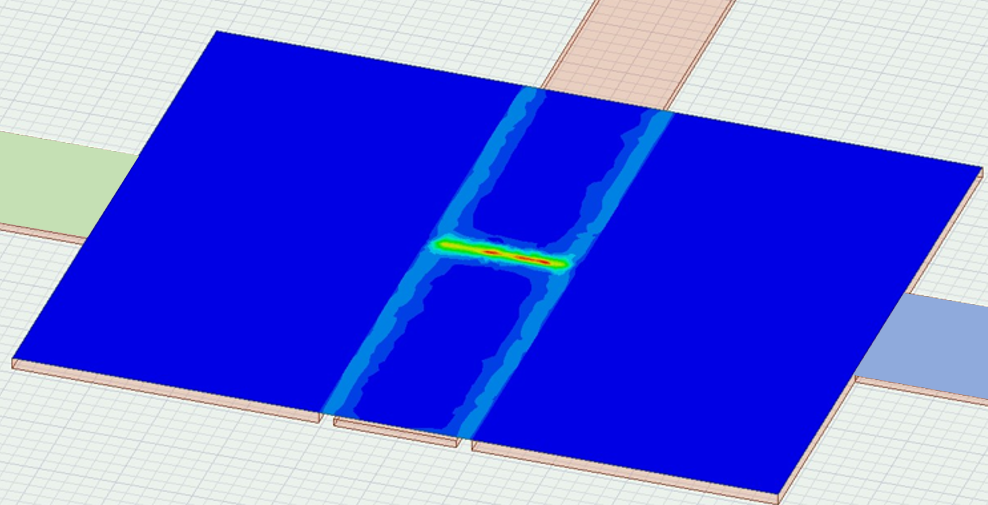
\includegraphics[width=0.7\textwidth]{Pic/Sim_NWcapa.png}
    \caption{The electric field distribution at the bottom cross-section of the nanowire (displayed in blue). The left and right orange pattern is the contact}
    \label{fig:my_label}
\end{figure}

Impedance matching is also an important consideration while designing the circuit. Almost all the instruments and cables are designed at impedance $Z = 50\Omega$ to minimize the signal reflection in connections.

\subsubsection{Grounded design}

The floating design is not suitable for gatemon since the gate tunes the Fermi energy of both the lead and the junction simultaneously, making it hard to adjust the $\omega_{01}$ of the qubits. Hence grounded design is used to ensure one lead has definite chemical potential. 


\begin{figure}[h!]
    \centering
    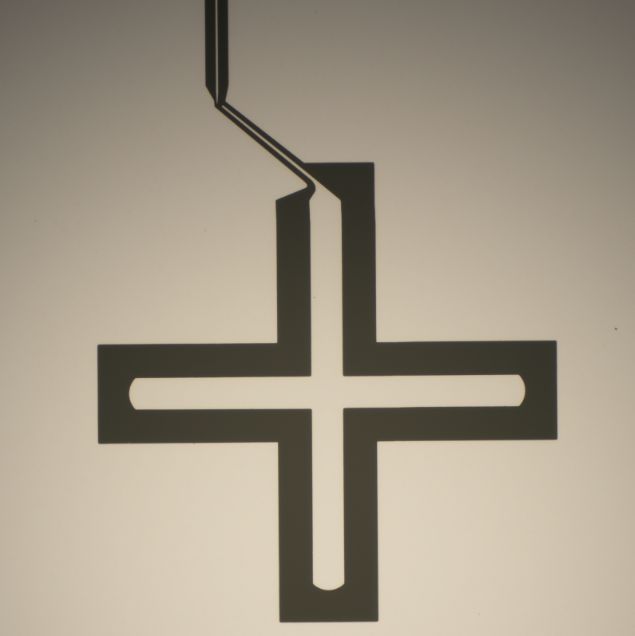
\includegraphics[width=0.5\textwidth]{Pic/Xmon_design.png}
    \caption{The X-mon grounding design.}
    \label{fig:my_label}
\end{figure}

The calculation now becomes:
\begin{equation}
    \begin{array}{cc}
    E_C =& e^2 / 2C_\Sigma \\
    \beta =& |\frac{C_\phi}{C_{coup}}| \\
    \hbar\omega_{01} =& \sqrt{8E_CE_J} - E_C
    \end{array}
\end{equation}


\subsection{Resonator design and simulation}
To measure multiple qubits through a transmission line (feedline) on the same chip, we need to carefully design the characteristic frequency of the resonators to avoid signal overlapping. The resonators are mutually coupled to the feedline and capacitively coupled to qubits, so it is a $\lambda/4$ resonator, and its frequency can be tuned by changing the distance of both ends. 

The resonator spectroscopy through VNA is read by $S_{21}$, defined as $V_2^-/V_1^+$, the voltage ratio of the reflected wave from port 2 to the incident wave into port 1. One important parameter in determining the goodness of resonators is quality factors\cite{RN65}:
\begin{equation}
    Q = \omega_0\frac{E_{tot}}{P_{loss}} = \frac{\omega_0}{\kappa}
\end{equation}
with $E_{tot}$ the total energy in the resonator and $P_{loss}$ the dissipated power. $\kappa$, the decay rate, namely the inverse of photon lifetime in the resonator, is defined as the full width at the half maximum (FWHM) of the Lorentzian shape response in the $S_{21}$ signal. The quality factor in the resonator can be further decomposed into internal and external (or coupling) quality factors:
\begin{equation}
\begin{array}{lrlrll}
     \frac{1}{Q}& =& \frac{1}{Q_i}& +& \frac{1}{Q_e}&  \\
     \kappa& =& \kappa_i& +& \kappa_e&
\end{array}
\end{equation}
$\kappa_i$ denotes the resonator spontaneous decay rate, and $\kappa_e$ denotes the decay to the environment and the transmission line. In practice, we design the value of $Q_e$ and constrain it in a reasonable interval to make a trade-off in the readout time and $T_1$ of the qubits.

We use HFSS to simulate the Q external quality factor by varying the distance between the feedline and the resonator. The estimated $Q_i$ is around 1 million, so the corresponding $Q_e$ should be more than 200-300 k. The resonance frequency is determined by the total length and shape of the resonator. To avoid the TWPA working frequency in our dilution fridge, we exclude the frequency at 6.6-6.75 GHz by design. In practice, the resonator's frequency might be shifted due to different materials and over or under-etched.

\subsection{Nanowires with shadow junction}

Our devices used in this thesis are all using In Situ growth shadow nanowires as SNS junctions to get highly transparent, clean interfaces. The Aluminum coat InAs/Sb nanowires are grown by Sabbir Khan with the series number Qdev 878\cite{RN38}, and Tantalum coat InAs nanowires are by T.Kanne with the number QDev 1226. We also use the Tantalum nanowires\cite{RN37} that are grown only for the N-S interface, but we can be lucky to find some nanowires that have S-N-S junctions.

\subsubsection{Aluminum coated nanowires with shadow junctions}
The Al shadowed nanowires are grown like crosses inside the trenches. Since the Al shadow wires are grown in purpose and the shadow junctions are formed with a high probability, there is no need to do SEM beforehand. We can pick the nanowires from one of the rows and quickly inspect them in SEM or AFM. 
\begin{figure}[h!]
    \centering
    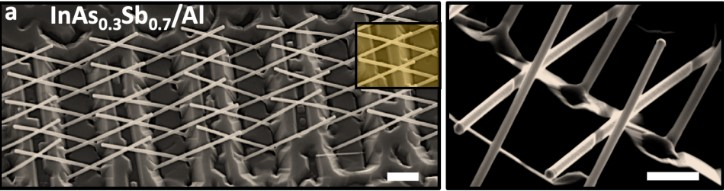
\includegraphics[width=0.85\textwidth]{Pic/AlShadowWire.jpg}
    \caption{The structure of the InAs$_{0.3}$Sb$_{0.7}$/Al shadow nanowires, picture from Sabbir's paper\cite{RN38} (scale bar is 500 nm)}
    \label{fig:my_label}
\end{figure}

This batch of nanowires is investigated heavily. These junctions can be tuned to a reasonably low critical current (10-15 nA) from many orders of MARs that show a low barrier on the S-N-S interface\cite{RN38}.

\subsubsection{Tantalum coated nanowires with shadow junctions}

However, the two Ta shadow nanowires' chips are in a different situation. Firstly, we need to go into SEM to locate the picking area we want. Then after proper rotation and tilt, we need to spend several hours in SEM to find wires with junctions and note them on paper. Then we move the chip to the micromanipulator and spend hours spotting and transferring the wires.
\begin{figure}[h!]
    \centering
    \begin{subfigure}[b]{0.48\textwidth}
         \centering
         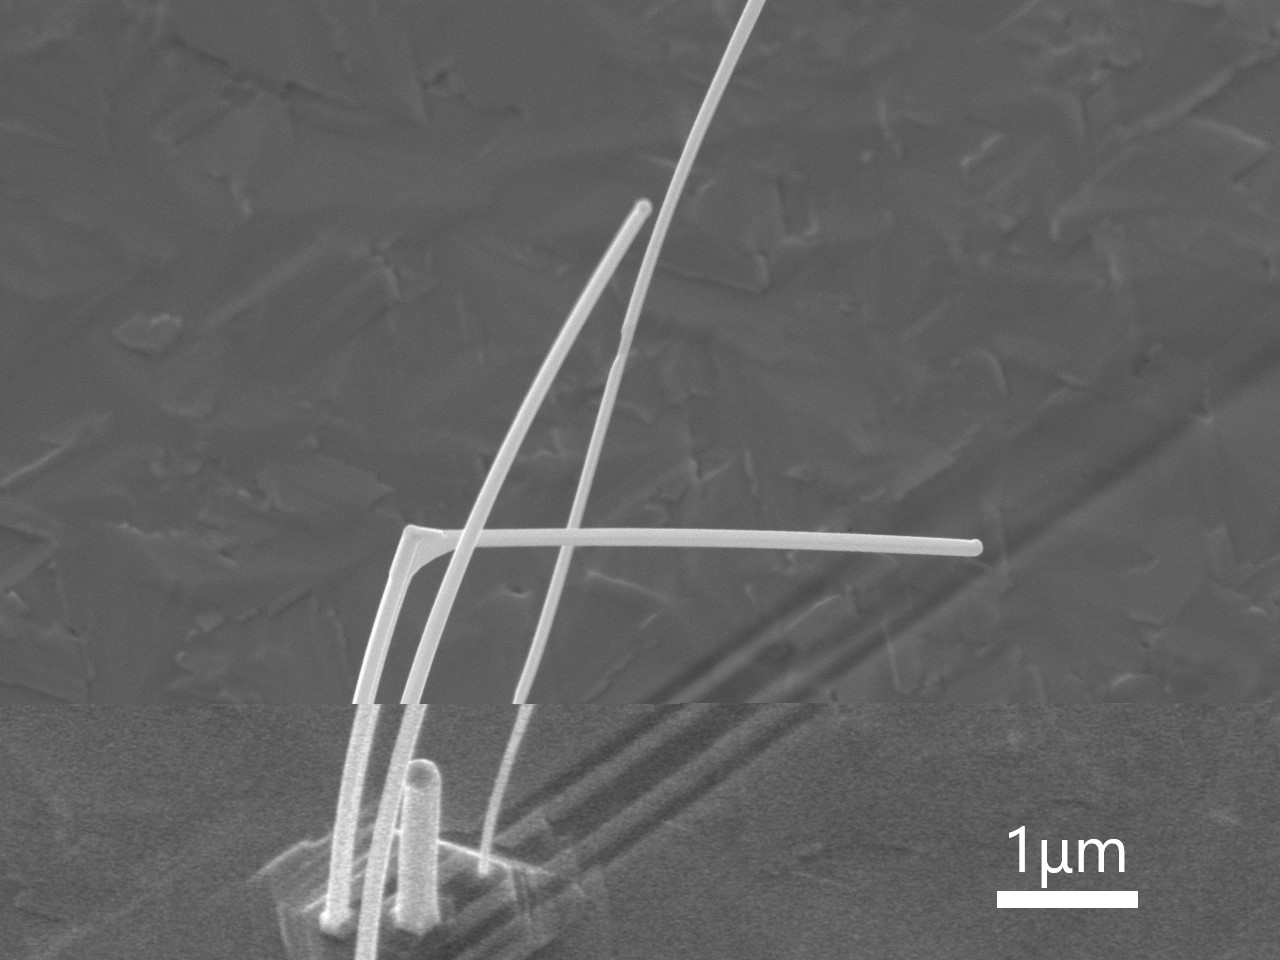
\includegraphics[width=\textwidth]{Pic/TaNWonChip.jpg}
         \caption{}
         \label{TaNWonchip}
     \end{subfigure}
     \hfill
     \begin{subfigure}[b]{0.48\textwidth}
         \centering
         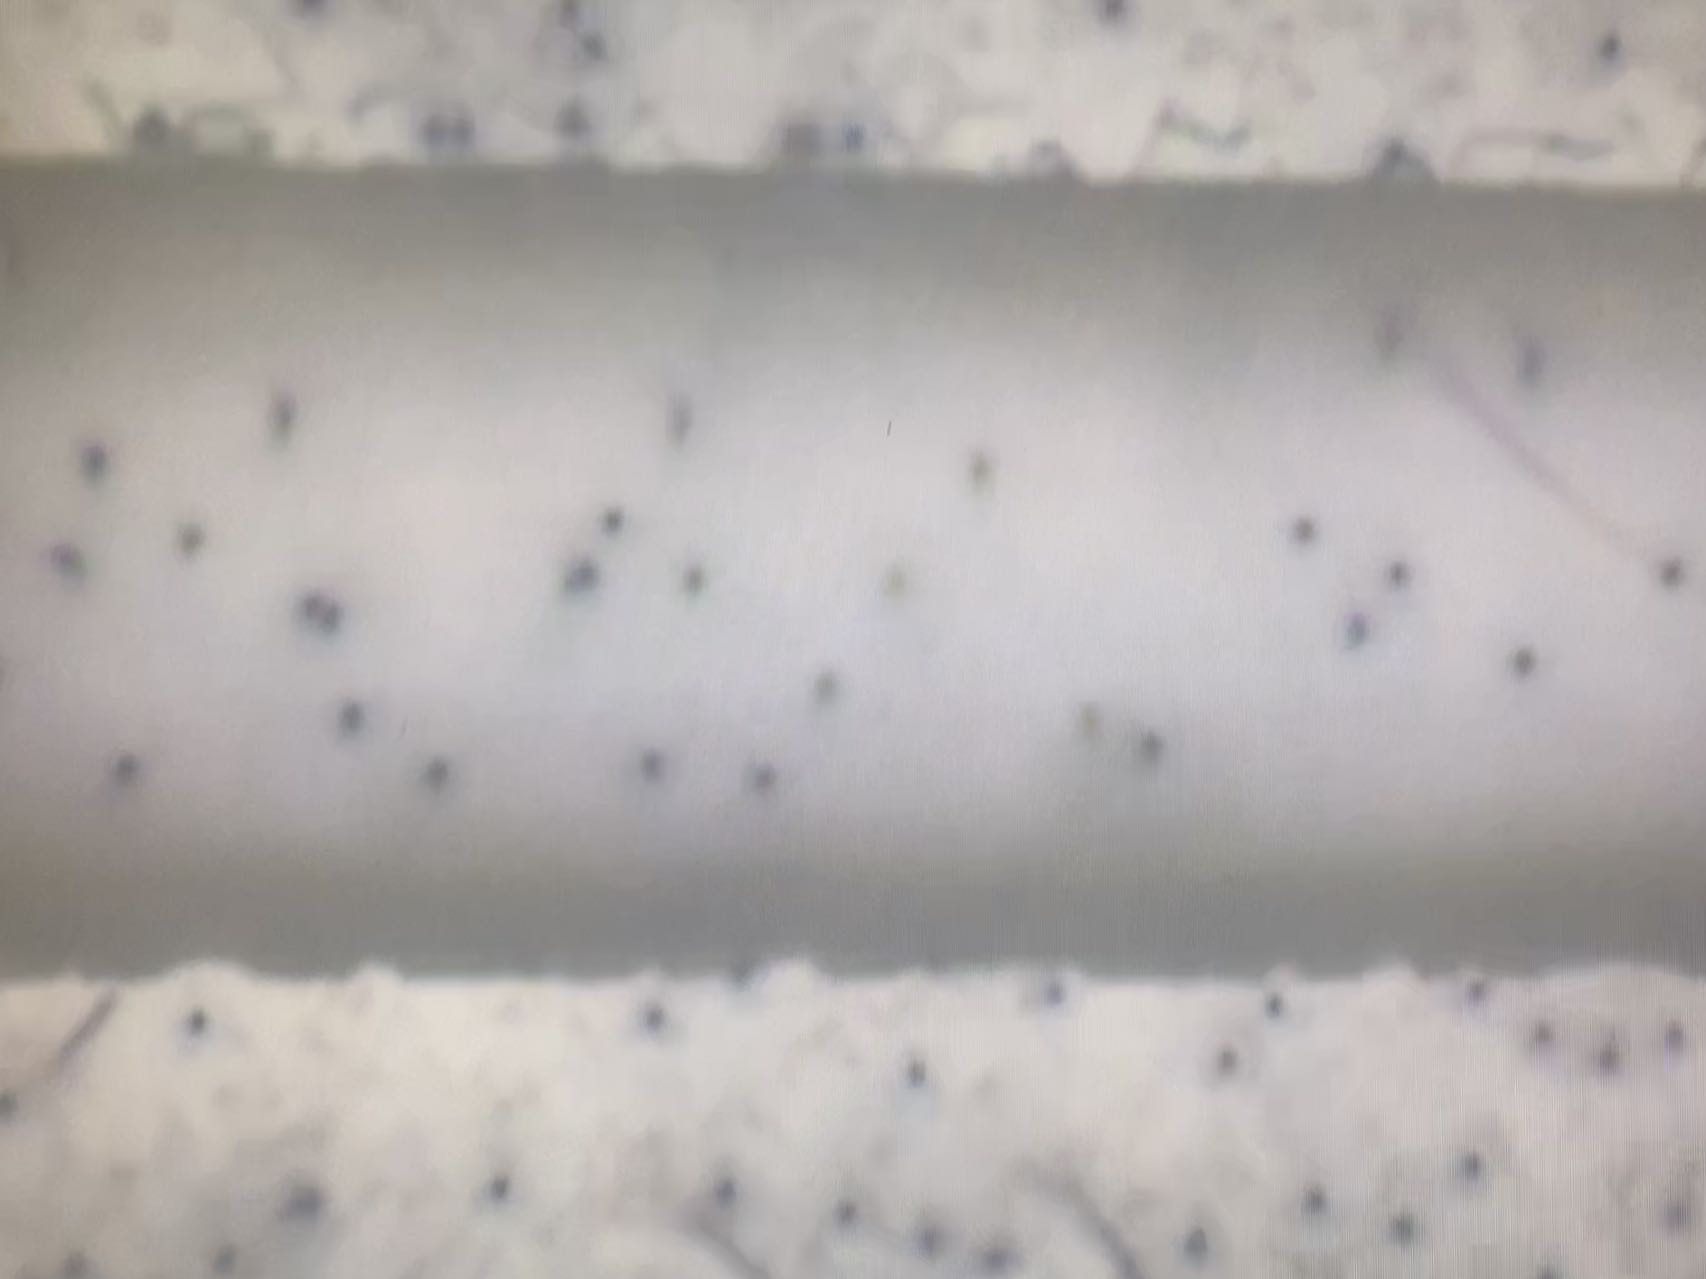
\includegraphics[width=\textwidth]{Pic/TaNWonChip2.jpg}
         \caption{}
         \label{fig:three sin x}
     \end{subfigure}
    \caption{(a) The nanowires on chip QDev 1226, with shadow junction. (b) In the view in the micromanipulator's microscope (on QDev 551) with 100x magnification, the black dot indicates a nanowire.}
    \label{TaNWonchip2}
\end{figure}

Because of the doping problem and potentially carbon contamination \cite{RN41}, it is necessary to reduce the gross time on nanowires and try to lower the applied voltage as low as possible. We occasionally use the SEM system JOEL 7800F, which can rotate the chip in all directions to find the junction better while facing down toward the substrate. An alternative, less charging solution is to use Raith eLine to do SEM. Since it has an alignment mark locating system, the nanowire can be found and photoed automatically in a short time. The system's downside is that it has no rotation motors, which might cause ambiguity when the junction face down. Besides, it locates in the cleanroom, so it takes us a long time to characterize the wires.

Most of the nanowires' inspections take less than 10 seconds, and gross inspection times less than 20 seconds. Sometimes due to the highly long nanowire and misfortune in the manipulator, the nanowires will be in SEM for a much longer time. 


\subsection{Aluminum based substrate chip fabrication and bonding}
The chips are diced 10x10 mm from Silicon(111) wafer with 100nm aluminum by E-beam evaporation in AJA or molecular beam epitaxy (MBE). The MBE aluminum has fewer impurities and defects than AJA aluminum due to the cleaner environment and finer control of film growth. Thus MBE aluminum has less two-level system (TLS), dangling bonds left on Metal-Air, and Metal-Substrate surface that are accelerating qubits' decoherence. However, AJA aluminum is easier and faster to grow. Therefore, we use AJA aluminum for nanowires transportation property measurement and MBE aluminum for high-frequency measurement in the dilution fridge.

The fabrication is divided into five steps: alignment marks, control line, gate half etch (or deposition), nanowires transfer, and contact deposition.

Alignment mark:
\begin{enumerate}
    \item Preclean: clean the chip in 1,3-dioxolane for 5 minutes, acetone for 5 minutes in sonication, and isopropyl alcohol (IPA) for 1 minute. Then dry the chip with nitrogen.
    \item Spin coat: Coated by PMMA A4 with 4000rpm, 45s spin and baked on $180^\circ$C hotplate for 2 minutes. Inspection in the bright field of the microscope that the coat is even except for the edge is recommended.
    \item Exposure: Load the chip into E-beam lithography ELS-F125, with dose 1000 $\mu$C/cm$^2$ and correct proximity effect correction (PEC) file.
    \item Development: Dip it into MIBK:IPA 1:3 solution for 1 minute to do development, then inspect under the bright and dark field in the microscope. Ash by oxygen for 1 minute to remove (around 8 nm) the remaining resist inside the trenches.
    \item Metal deposition: Load it into E-beam evaporation (AJA) to deposit 5nm Ti seed layer and 40nm Au.
    \item Liftoff: Soak the chip into acetone for 30 minutes to lift off the resist with metal. 
\end{enumerate}

The control line process is similar to the alignment marks process in the first half, but after the development:

\begin{enumerate}
    \item Postbake: Rest the chip for 2 minutes on the $115^\circ$C hot plate in order to harden the resist. 
    \item Etching: Dip the chip into $50^\circ$C of Transene Aluminum Etchant Type-D (TranseneD) for around 23 seconds (AJA aluminum) or 25 seconds (MBE aluminum) with slow agitation, then immediately soak it into $50^\circ$C milliQ for 20s and room temperature milliQ for 40s. Check under the microscope to see whether it is under-etched. If yes, redo the etching step but reduce the time in TranseneD to 3-5 seconds.
    \item Strip: Soak the chip into acetone for 10 minutes to remove the resist.
\end{enumerate}

Now, if 1. we want a half-etched gate, we can do the same as the control line process except for the around 8s aluminum etch in TranseneD during the etching step. This gate will separate the nanowire physically well from the bottom gate. 2. The other alternative process is depositing a 6nm Hafnium oxide ALD layer on top of the gate without etching. This method is targeted to increase the electric field strength felt by junctions and make them easier to pinch off. We will discuss this later in the result.

\begin{figure}[h!]
    \centering
    \begin{subfigure}[b]{0.45\textwidth}
         \centering
         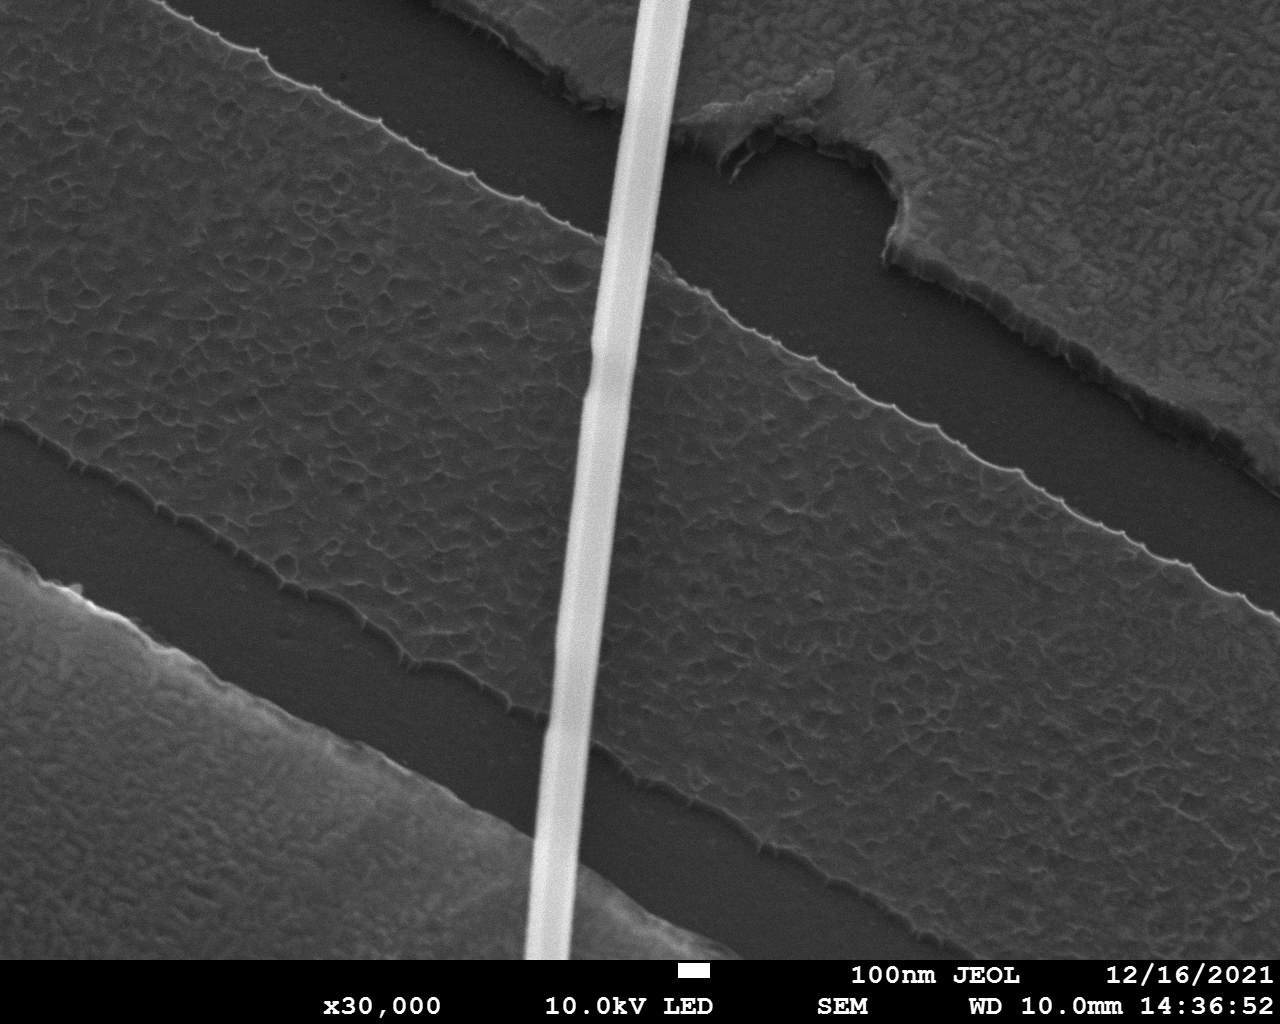
\includegraphics[width=\textwidth]{Pic/Gatehalfetch.jpg}
         \caption{}
         \label{halfetchgate}
     \end{subfigure}
     \hfill
     \begin{subfigure}[b]{0.45\textwidth}
         \centering
         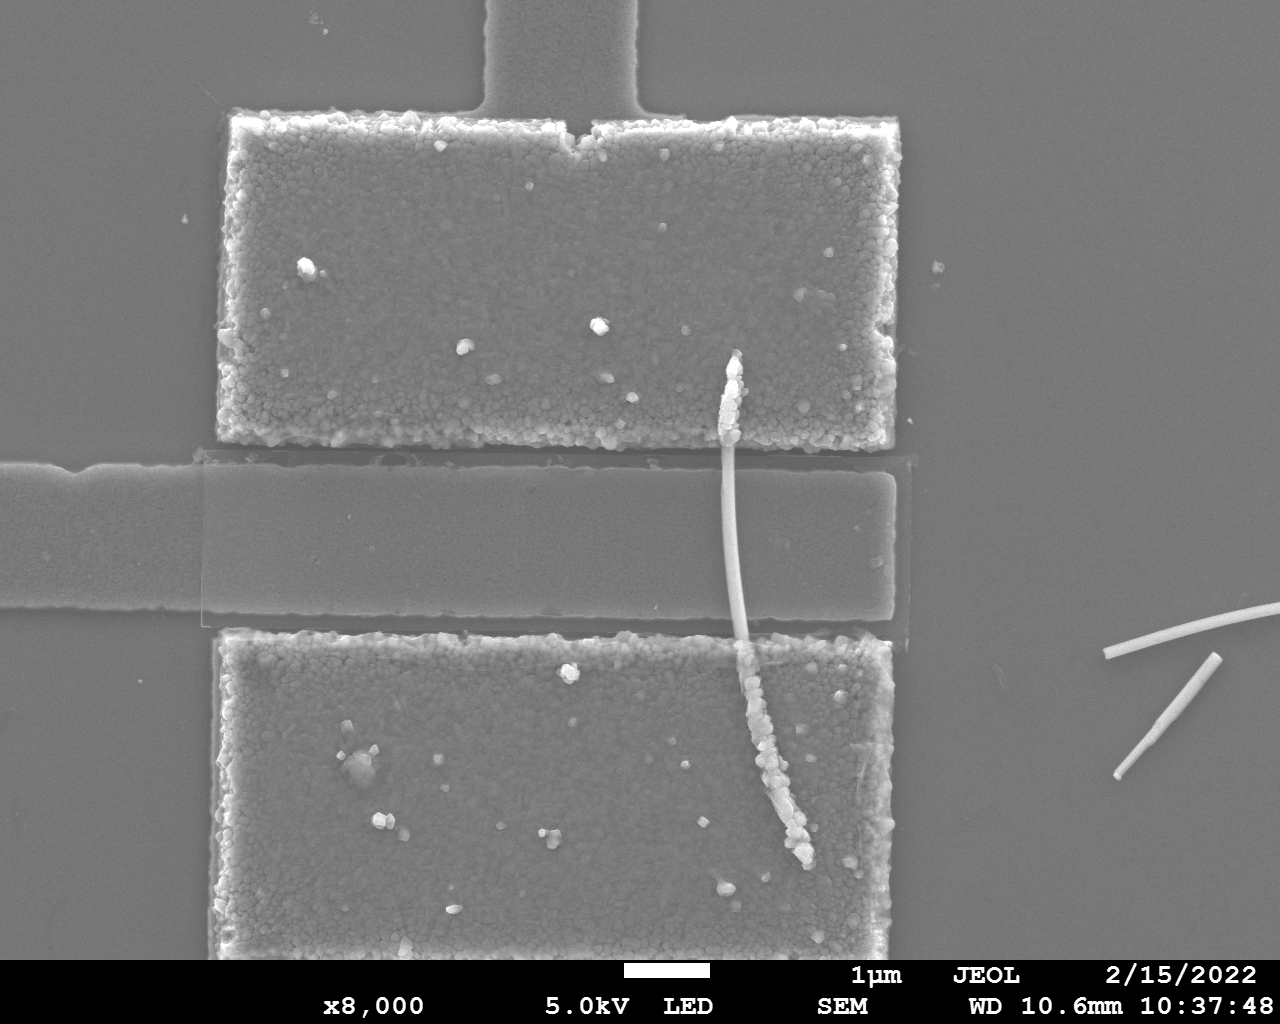
\includegraphics[width=\textwidth]{Pic/ALDlayer.jpg}
         \caption{}
         \label{fig:three sin x}
     \end{subfigure}
    \caption{Left figure is the gate with half etch and right is the gate with direct deposition of 6nm ALD layer}
    \label{ALDgate}
\end{figure}

Then the chip is transferred to the micro-manipulator, and we use 0.1-micrometer Tungsten tips to move the nanowires to the chip. Since the junctions are too small to see in the optical microscope, we usually use SEM to do a quick scan on nanowires and then go back and forth until we make all the junctions located above the gates. However, we discover that SEM will inject impurities and defects into the semiconductor and thus make the junction more conductive, with less probability of pinching off. One way to circumvent this issue is to use AFM to sense the location of the junction. It is experimentally successful sometimes, but it is also very likely to move the nanowire to a random place on the chip through Van der Waals force. Another solution provided is to use an optical surface profilometer to do harmless detection of junctions. We will try this method in our future development.

The final step is contact deposition. Since the nanowires can't withstand temperature at $180^\circ$C, we instead use $115^\circ$C to bake the resist:
\begin{enumerate}
    \item Spin coat: First, we do EL9 with 4000rpm / 45 seconds, then $115^\circ$C baking on the hotplate. Then one more layer of EL9 and one layer of PMMA A4 with the same procedure. In total, three layers of resist are spun.
    \item Exposure: Load the chip into ELS-F125 with dose 1000 $\mu$C/cm$^2$.
    \item Development: Soak into MIBK:IPA 1:3 solution for 1 minute, then inspect under the bright and dark field in the microscope. Ash by oxygen for 1 minute.
    \item DC milling: Load it into E-beam evaporation (AJA), use Kaufman ion milling (DC milling) with 300 V, 15 SCCM airflow, and 0.41 mbar for 1 minute to bombard the insulating oxidation layer.
    \item Metal deposition: Deposit 300-400 nm aluminum with $1 \text{\AA} / s$.
    \item Liftoff: Soak the chip into acetone overnight. 
\end{enumerate}

The bonding process depends on which board we are using. If we are using Copenhagen board v7p1 or v8p0 for DC measurement, then use PMMA A4 to glue the chip on the daughterboard and use F/S Bondtec 5630 bonder to connect the port and the chip. Finally, take an overall picture of the board, and then the daughterboard with the chip is ready to load into the fridge and undergo measurement.

\subsection{Tantalum based substrate fabrication}

Recent research \cite{RN26, RN67} demonstrates supreme performance on tantalum-based transmon, which can reach a 0.5 millisecond lifetime. As a consequence, tantalum probably is a great material for building a gatemon.

We ordered a 100 nanometers thick Tantalum on a $430\mu m$single-side polished sapphire wafer from Star Cryoelectronics and diced it to 10x10 mm at Technical University of Denmark (DTU). The etchant we use is Transene 111 ($\text{HF:HNO}_3\text{:H}_2\text{O = 1:1:1})$. While doing the exposure on sapphire, we need to scratch and fix the metal clamp at the edge of the chip to form direct contact with the metal on top of the substrate. Aside from this detail, the alignment mark process is the same as the aluminum substrate. 

\begin{figure}[h!]
    \centering
    \begin{subfigure}[b]{0.47\textwidth}
         \centering
         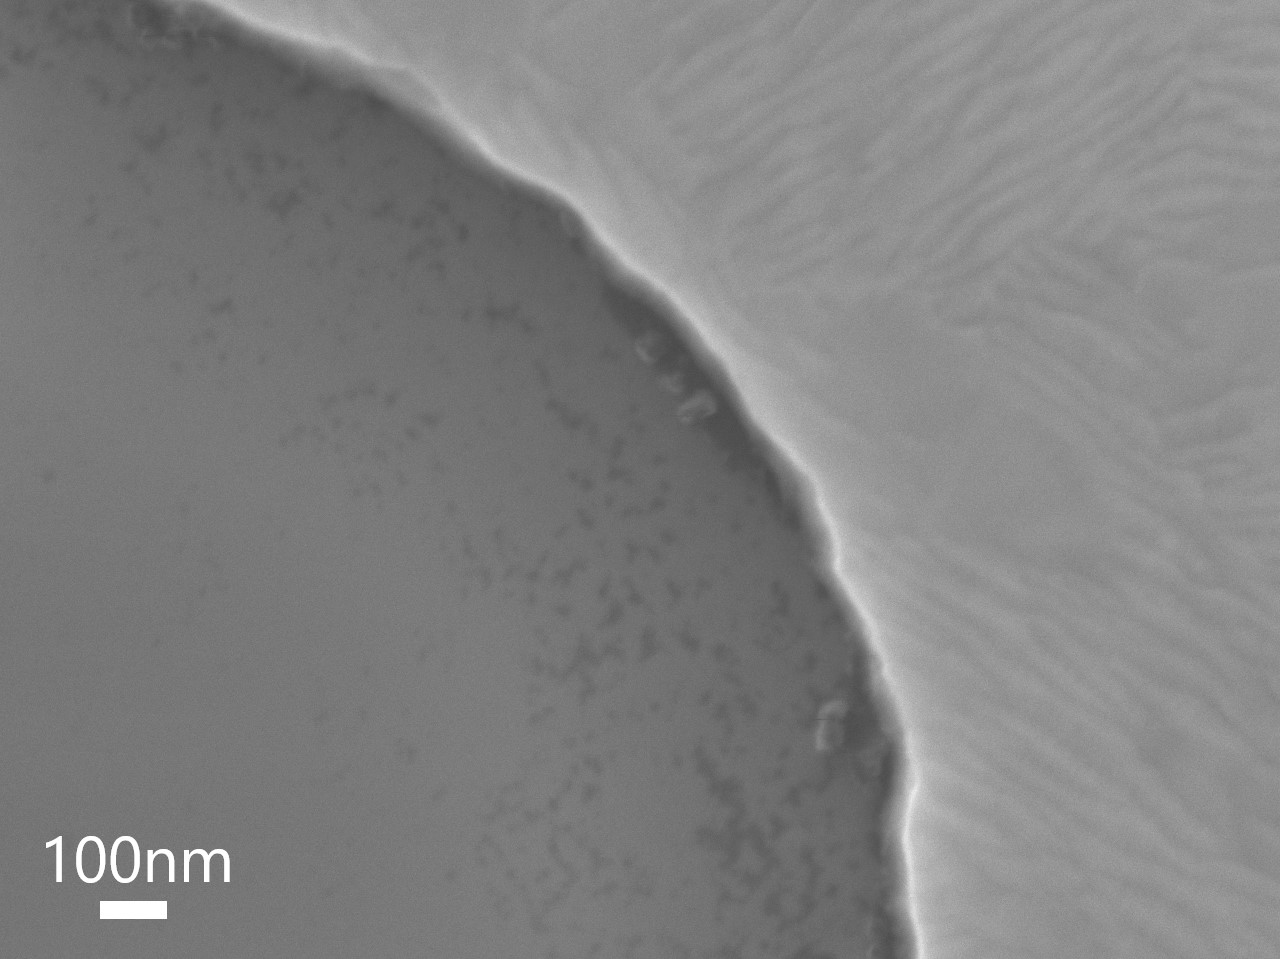
\includegraphics[width=\textwidth]{Pic/TaEtch_0.jpg}
         \caption{}
         \label{halfetchgate}
     \end{subfigure}
     \hfill
     \begin{subfigure}[b]{0.47\textwidth}
         \centering
         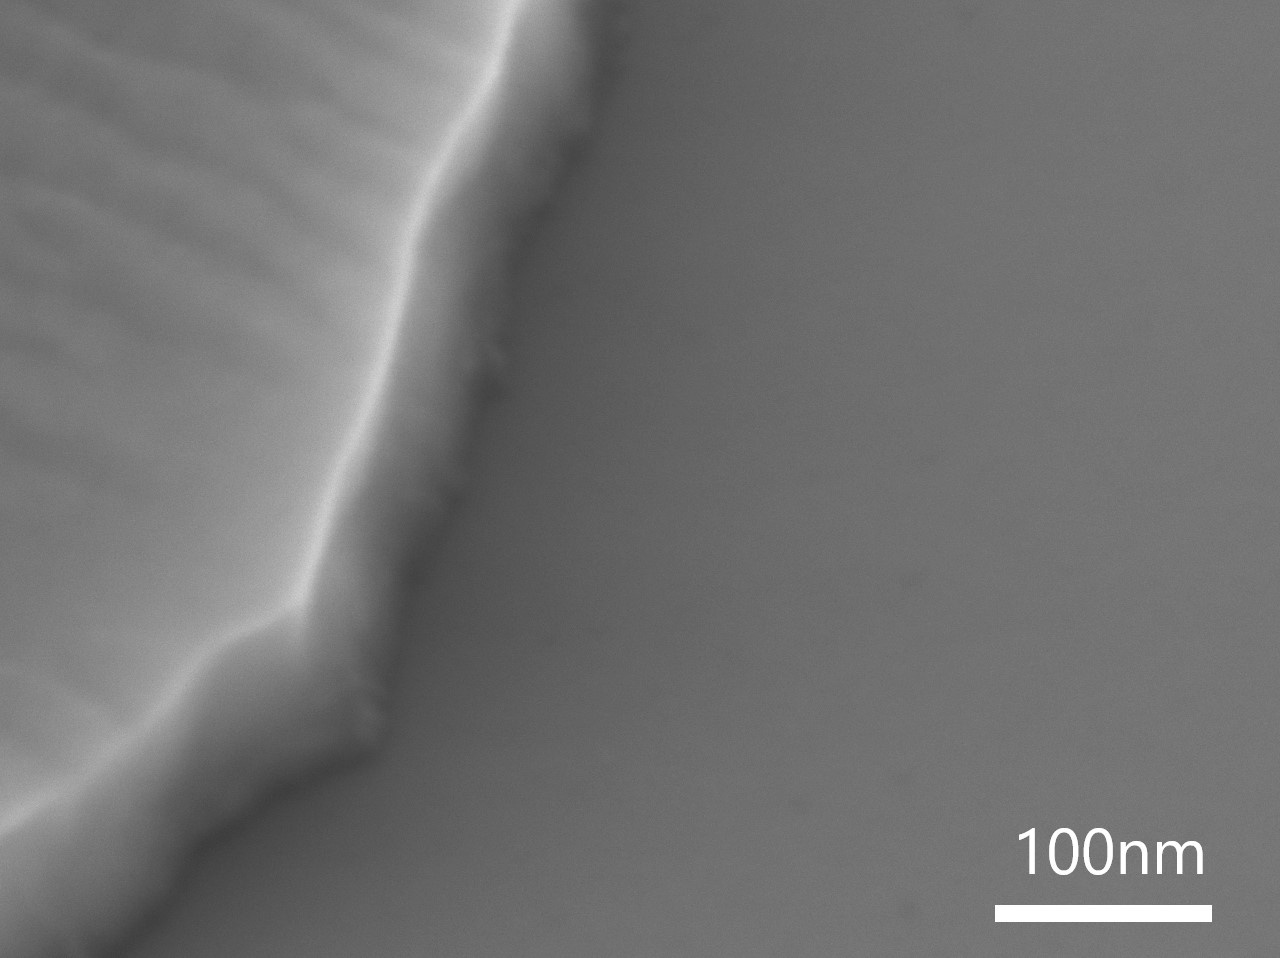
\includegraphics[width=\textwidth]{Pic/TaEtch.jpg}
         \caption{}
         \label{fig:three sin x}
     \end{subfigure}
    \caption{(a) The dots on the deep grey part shows that the etchant slightly attacks the substrate. (b) The etching leaves a sharp edge on tantalum.}
    \label{ALDgate}
\end{figure}

The etchant containing a high concentration of nitric acid and hydrofluoric acid makes it hard to use E-beam resist on etching (see Appendix B for more detail). Thus, we use photo-lithography instead of e-beam lithography:

\begin{enumerate}
    \item Spin coat: Use the pipette to drop AZ 5214E on the chip, and spin it at 4000 rpm / 45 seconds, then bake for 50 seconds on $110^\circ$C hotplate. Check the resist under the microscope with the yellow and green light filter to prevent pre-exposure on the resist.
    \item Lithography: Load the chip into Heidelberg µPG 501 ultra-violet photolithography system. Set the defocus to 2 and dose to 30 ms.
    \item Development: Fill a small size plastic beaker with AZ DEV (1:1). Develop the chip for 45 seconds with slow stirring for 3 seconds, and then rinse it into MilliQ for 30 seconds. Check under the dark-field microscope to see if any resist is left on the trenches (very important). Redo the lithography if there are many unwanted dots in the pattern. Then ash the chip for 2 minutes.
    \item Etching: Postbake the chip on $120^\circ$C hotplate. Etch tantalum in room temperature Transene111 for 8 seconds with slow stirring (2 seconds per round). Then we rinse the chip into two beakers of MilliQ respectively for 20 seconds and 40 seconds.
    \item Strip: Rinse the chip into 1,3-dioxolane for 10 minutes, acetone for 5 minutes, and MilliQ for 1 minute.
\end{enumerate}

It is not recommended to use IPA in the last step since we have several reports on contamination left on the chip after using it, but never for MilliQ. 

The ALD layer deposition is similar to the process on the aluminum substrate. However, to form a discharge layer on the floating patterns, we need to deposit a 15 nm aluminum layer on top of the resist before going into lithography. Remember to use the clamp on the discharge layer. After the exposure, we simply soak the chip into MF321 for 60 seconds, rinse it with MilliQ for 60 seconds and dry it. After confirming the disappearance of aluminum, the remaining development and ALD layer forming is the same as the previous one. 

Contacts deposition also needs an extra discharge layer on top of the chip:
\begin{enumerate}
    \item Spin coat: Two layers of EL9 and one layer of PMMA A4 with 4000rpm / 45 seconds and $115^\circ$C baking on the hotplate.
    \item Discharge layer: Deposit 15 nm of aluminum on the resist in the AJA system. 
    \item Exposure: Load the chip into ELS-F125 with dose 1000 $\mu$C/cm$^2$ with a clamp on the discharge layer.
    \item Etch discharge layer: Immerse the chip into MF321 for 60 seconds to fully etch out the aluminum, then rinse it with MilliQ for 60 seconds.
    \item Development: Soak into MIBK:IPA 1:3 solution for 1 minute, then inspect under bright and dark field in the microscope. Ash by oxygen for 1 minute.
    \item DC milling: Load it into the AJA system, use Kaufman ion milling with 300 V, 15 SCCM air flow, and 0.41 mbar for 1 minute to bombard the insulating oxidation layer.
    \item Metal deposition: Deposit 300 nm aluminum with $1 \text{\AA} / s$.
    \item Liftoff: Soak the chip in acetone for more than 3 hours. Dry it after dipping into IPA for 30 seconds. 
\end{enumerate}

The edge on the tantalum pattern looks sharp, and the sapphire substrate is slightly attacked. 


\subsection{Board station setup}

The board station is one cryogenic environment that we used mainly for testing the gate function on the chips. The model is CRX-4K Cryogenic Probe Station from Lake Shore, and the base temperature goes down to around 5 K on the temperature gauge.

\begin{figure}
    \centering
    \begin{subfigure}[b]{0.51\textwidth}
         \centering
         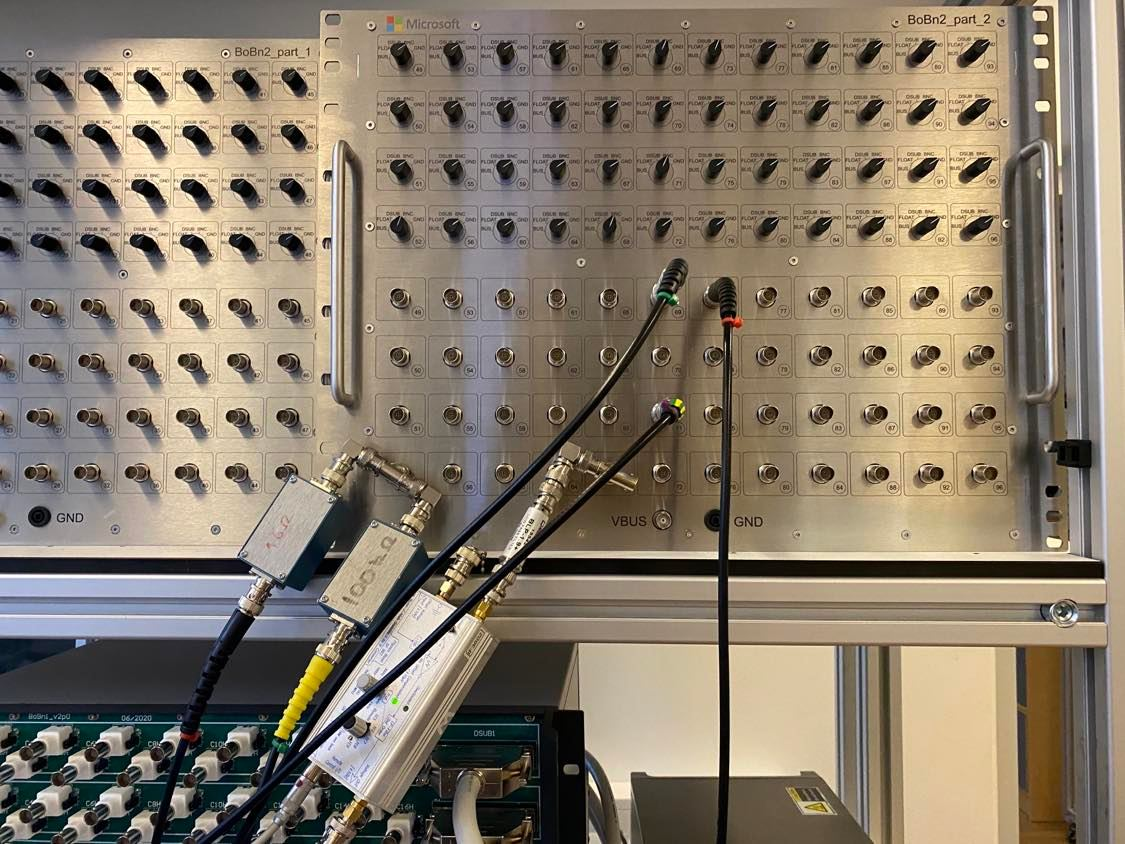
\includegraphics[width=\textwidth]{Pic/4KBoB.jpg}
         \caption{}
         \label{TaNWonchip}
     \end{subfigure}
     \hfill
     \begin{subfigure}[b]{0.45\textwidth}
         \centering
         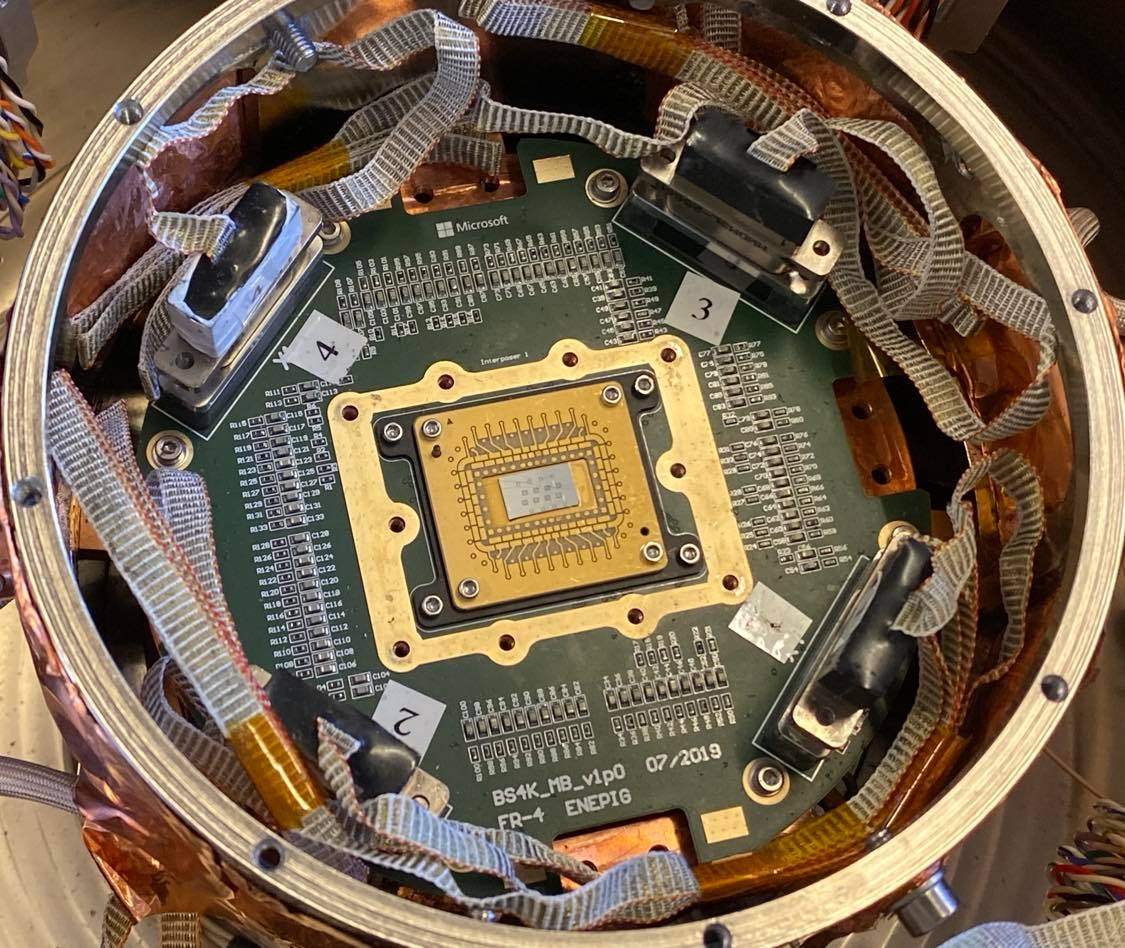
\includegraphics[width=\textwidth]{Pic/Chipin4K.jpg}
         \caption{}
         \label{fig:three sin x}
     \end{subfigure}
    \caption{(a) The breakout box used to connect to the instruments for measurement. (b)The chip is loaded into the board station. The probe arms are all removed to lower the base temperature of the apparatus.}
    \label{fig:my_label}
\end{figure}

The port on the daughterboard is connected to the breakout box. The fully cool down time of this station is less than 3 hours. Therefore it is truly convenient to test connectivity, gate functionality, and leakage in this system.

\subsection{Dilution refrigerator setup}

The dilution refrigerator is one of the most significant systems in our measurement. Its core physics process is the change of concentration of the Fermi gas like $^3\text{He}$ from dilute phase Bose statistics $^4\text{He}$ (More details in Pobell's textbook\cite{RN69}). The cool-down operation has two stages: the first stage is called precooling, which takes the gas state of $^3\text{He}$-$^4\text{He}$ mixture into a pulse tube cooler and circulates in the mixing chamber, the final coldest part in the fridge. When the mixing chamber reaches 10 K, condensing process starts. The $^3\text{He}$ is continuously pumping into the mixing chamber, maintaining the 6.4\% $^3\text{He}$ in $^4\text{He}$ rich phase inside. The still pump then keeps pumping the $^3\text{He}$ out from $^4\text{He}$ in the distiller (still) due to the lower latent heat, thus a higher vapor pressure of $^3\text{He}$. Different concentration leads to an osmotic pressure $\Delta \pi$ between the mixing chamber and still, which 'sucks' $^3\text{He}$ to the still. The heat exchanger in between them is cooling down the returning $^3\text{He}$. Theoretically, the mixing chamber can reach 10 mK by using this method.

\begin{figure}[h!]
    \centering
    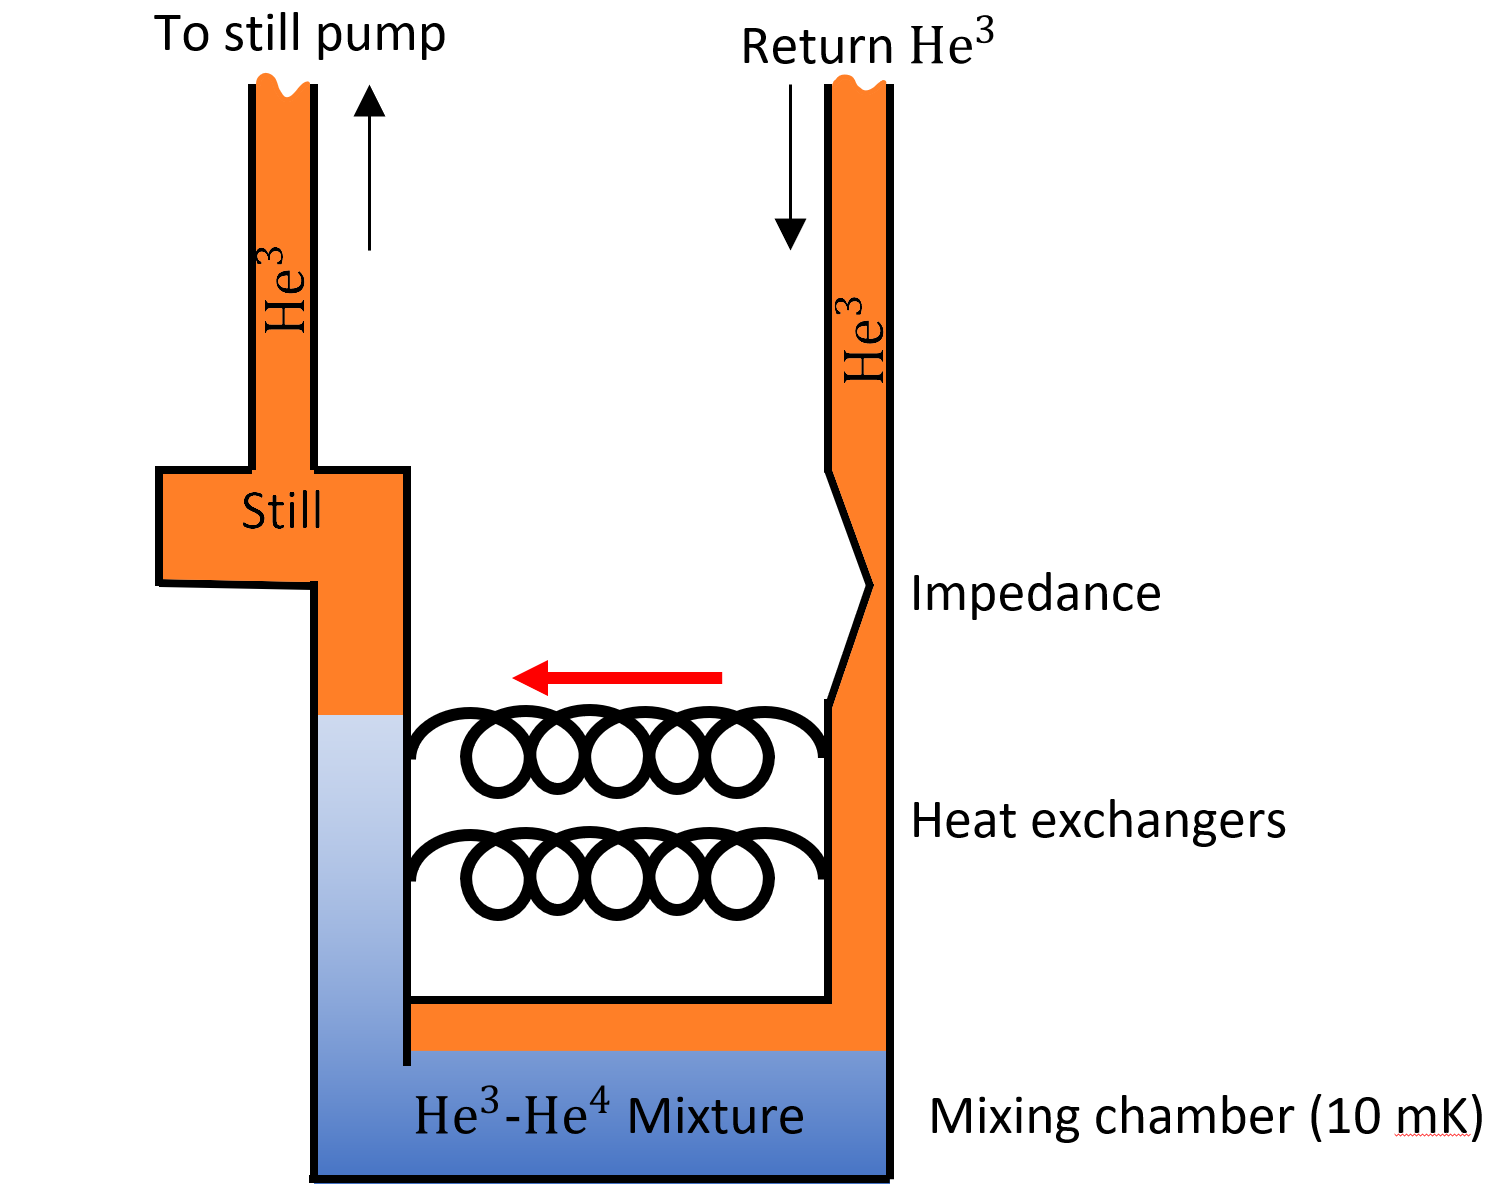
\includegraphics[width=0.7\textwidth]{Pic/MixingChamber.png}
    \caption{The mixing chamber and the distiller (still) in the dilution fridge. The impedance is used to condense the returning $^3\text{He}$ by Joule-Thompson expansion combined with the heat exchangers.}
    \label{fig:my_label}
\end{figure}

The cryogenic environment in the fridge can enable the superconducting state of aluminum and tantalum on the chip, maintaining a high vacuum and suppressing the circuit's thermal excitation. Moreover, it is also responsible for filtering the external mechanical vibration and shielding the exterior electromagnetic wave.

\begin{figure}[h!]
    \centering
    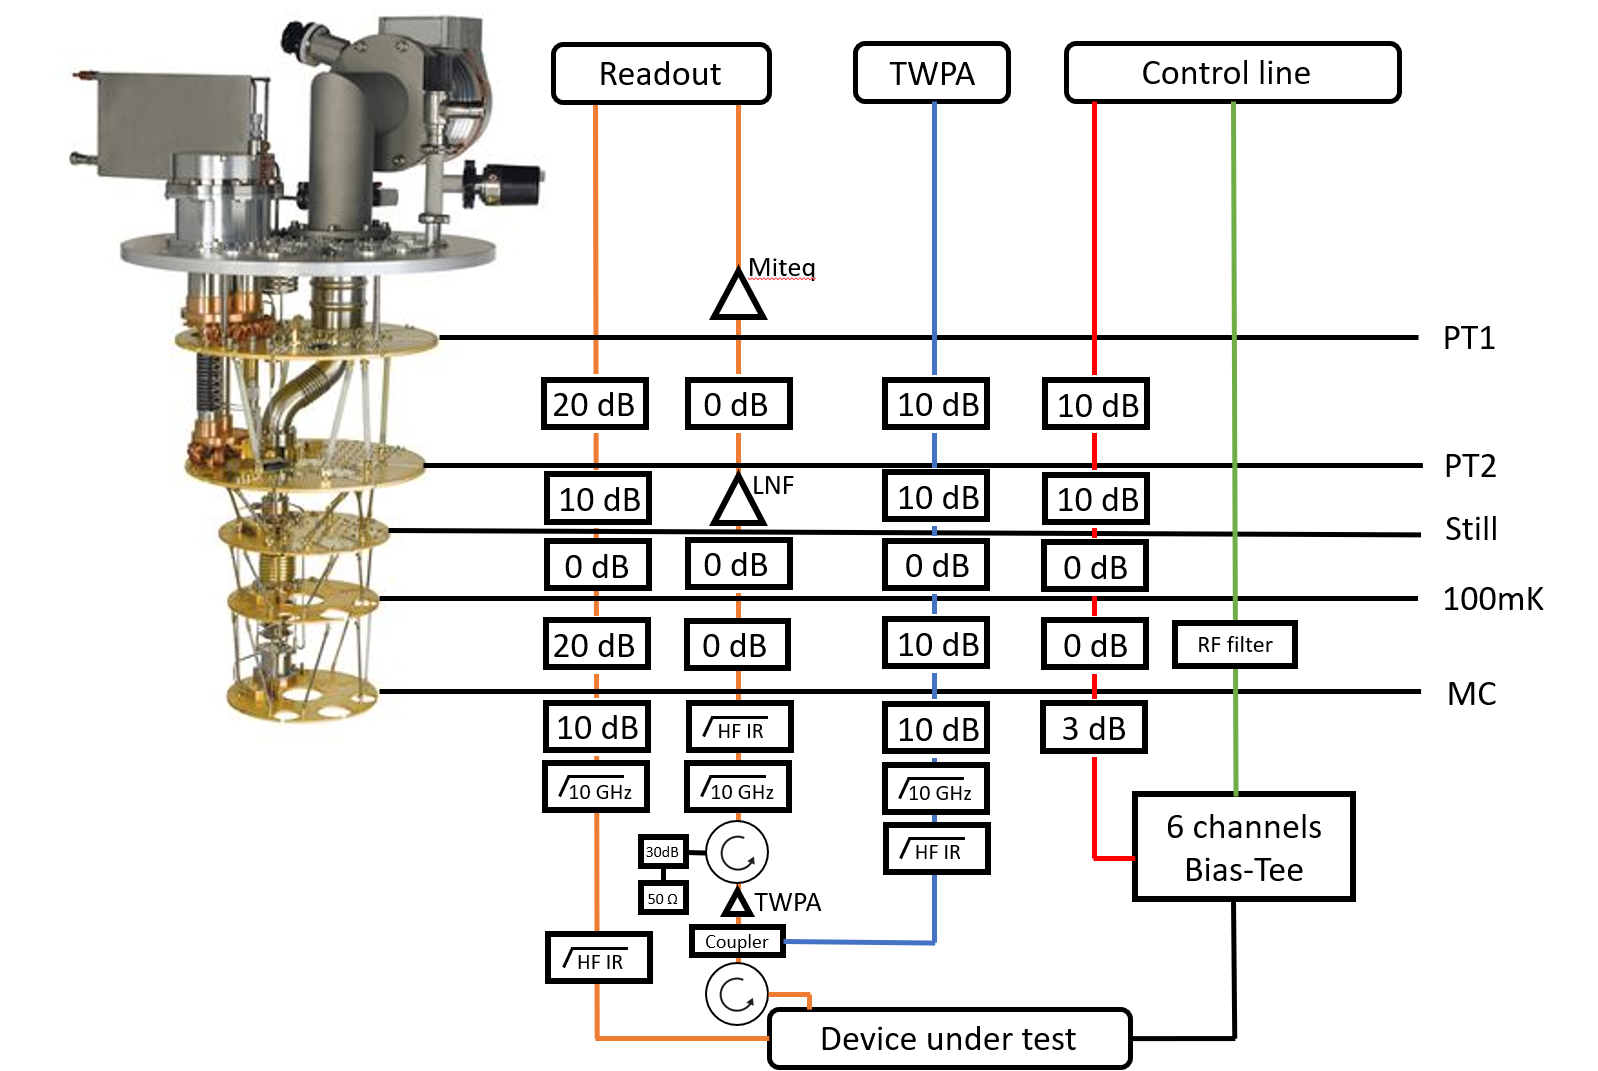
\includegraphics[width=\textwidth]{Pic/FridgeSetup.png}
    \caption{Wiring of T2 dilution fridge in QDev. The orange line is the readout line (the left goes into the device, and the right goes out). The red line is the high-frequency drive line for qubit control, and the green one is the DC line for gating.}
    \label{T2wiring}
\end{figure}

The fridge we use is Triton 200 from Oxford Instrument, with a base temperature of 23 mK with our samples loaded. The wiring is shown in Fig \ref{T2wiring}. Besides the DC gate line connected to the bias-tee, there is a 24 ports DC loom with nano-D connectors linking directly to the motherboard for transportation measurement purposes. The DC lines are connected to the breakout box (BoB), the integrated board with the ground, float, and bus function on each port. The apparatuses are connected to the BoB through BNC cables for DC and SMA connector coaxial lines for high-frequency measurements. The in-going readout signal experiences 60 dB attenuation (more in the experiment. See Chapter 5) and a high-frequency filter. The out-going readout signal is subsequently amplified by superconducting traveling wave parametric amplifier (TWPA)\cite{RN70}, high-electron-mobility transistor (HEMT) from Low Noise Factory (LNF) LNC4\_8C616Z and room temperature amplifier Miteq. All the readout lines are mounted with a high-frequency infrared filter to absorb the unwanted 20 GHz to hundreds of THz light, excluding the extract heat source along the coaxial cable.


\begin{figure}[h!]
    \centering
    \begin{subfigure}[b]{0.45\textwidth}
         \centering
         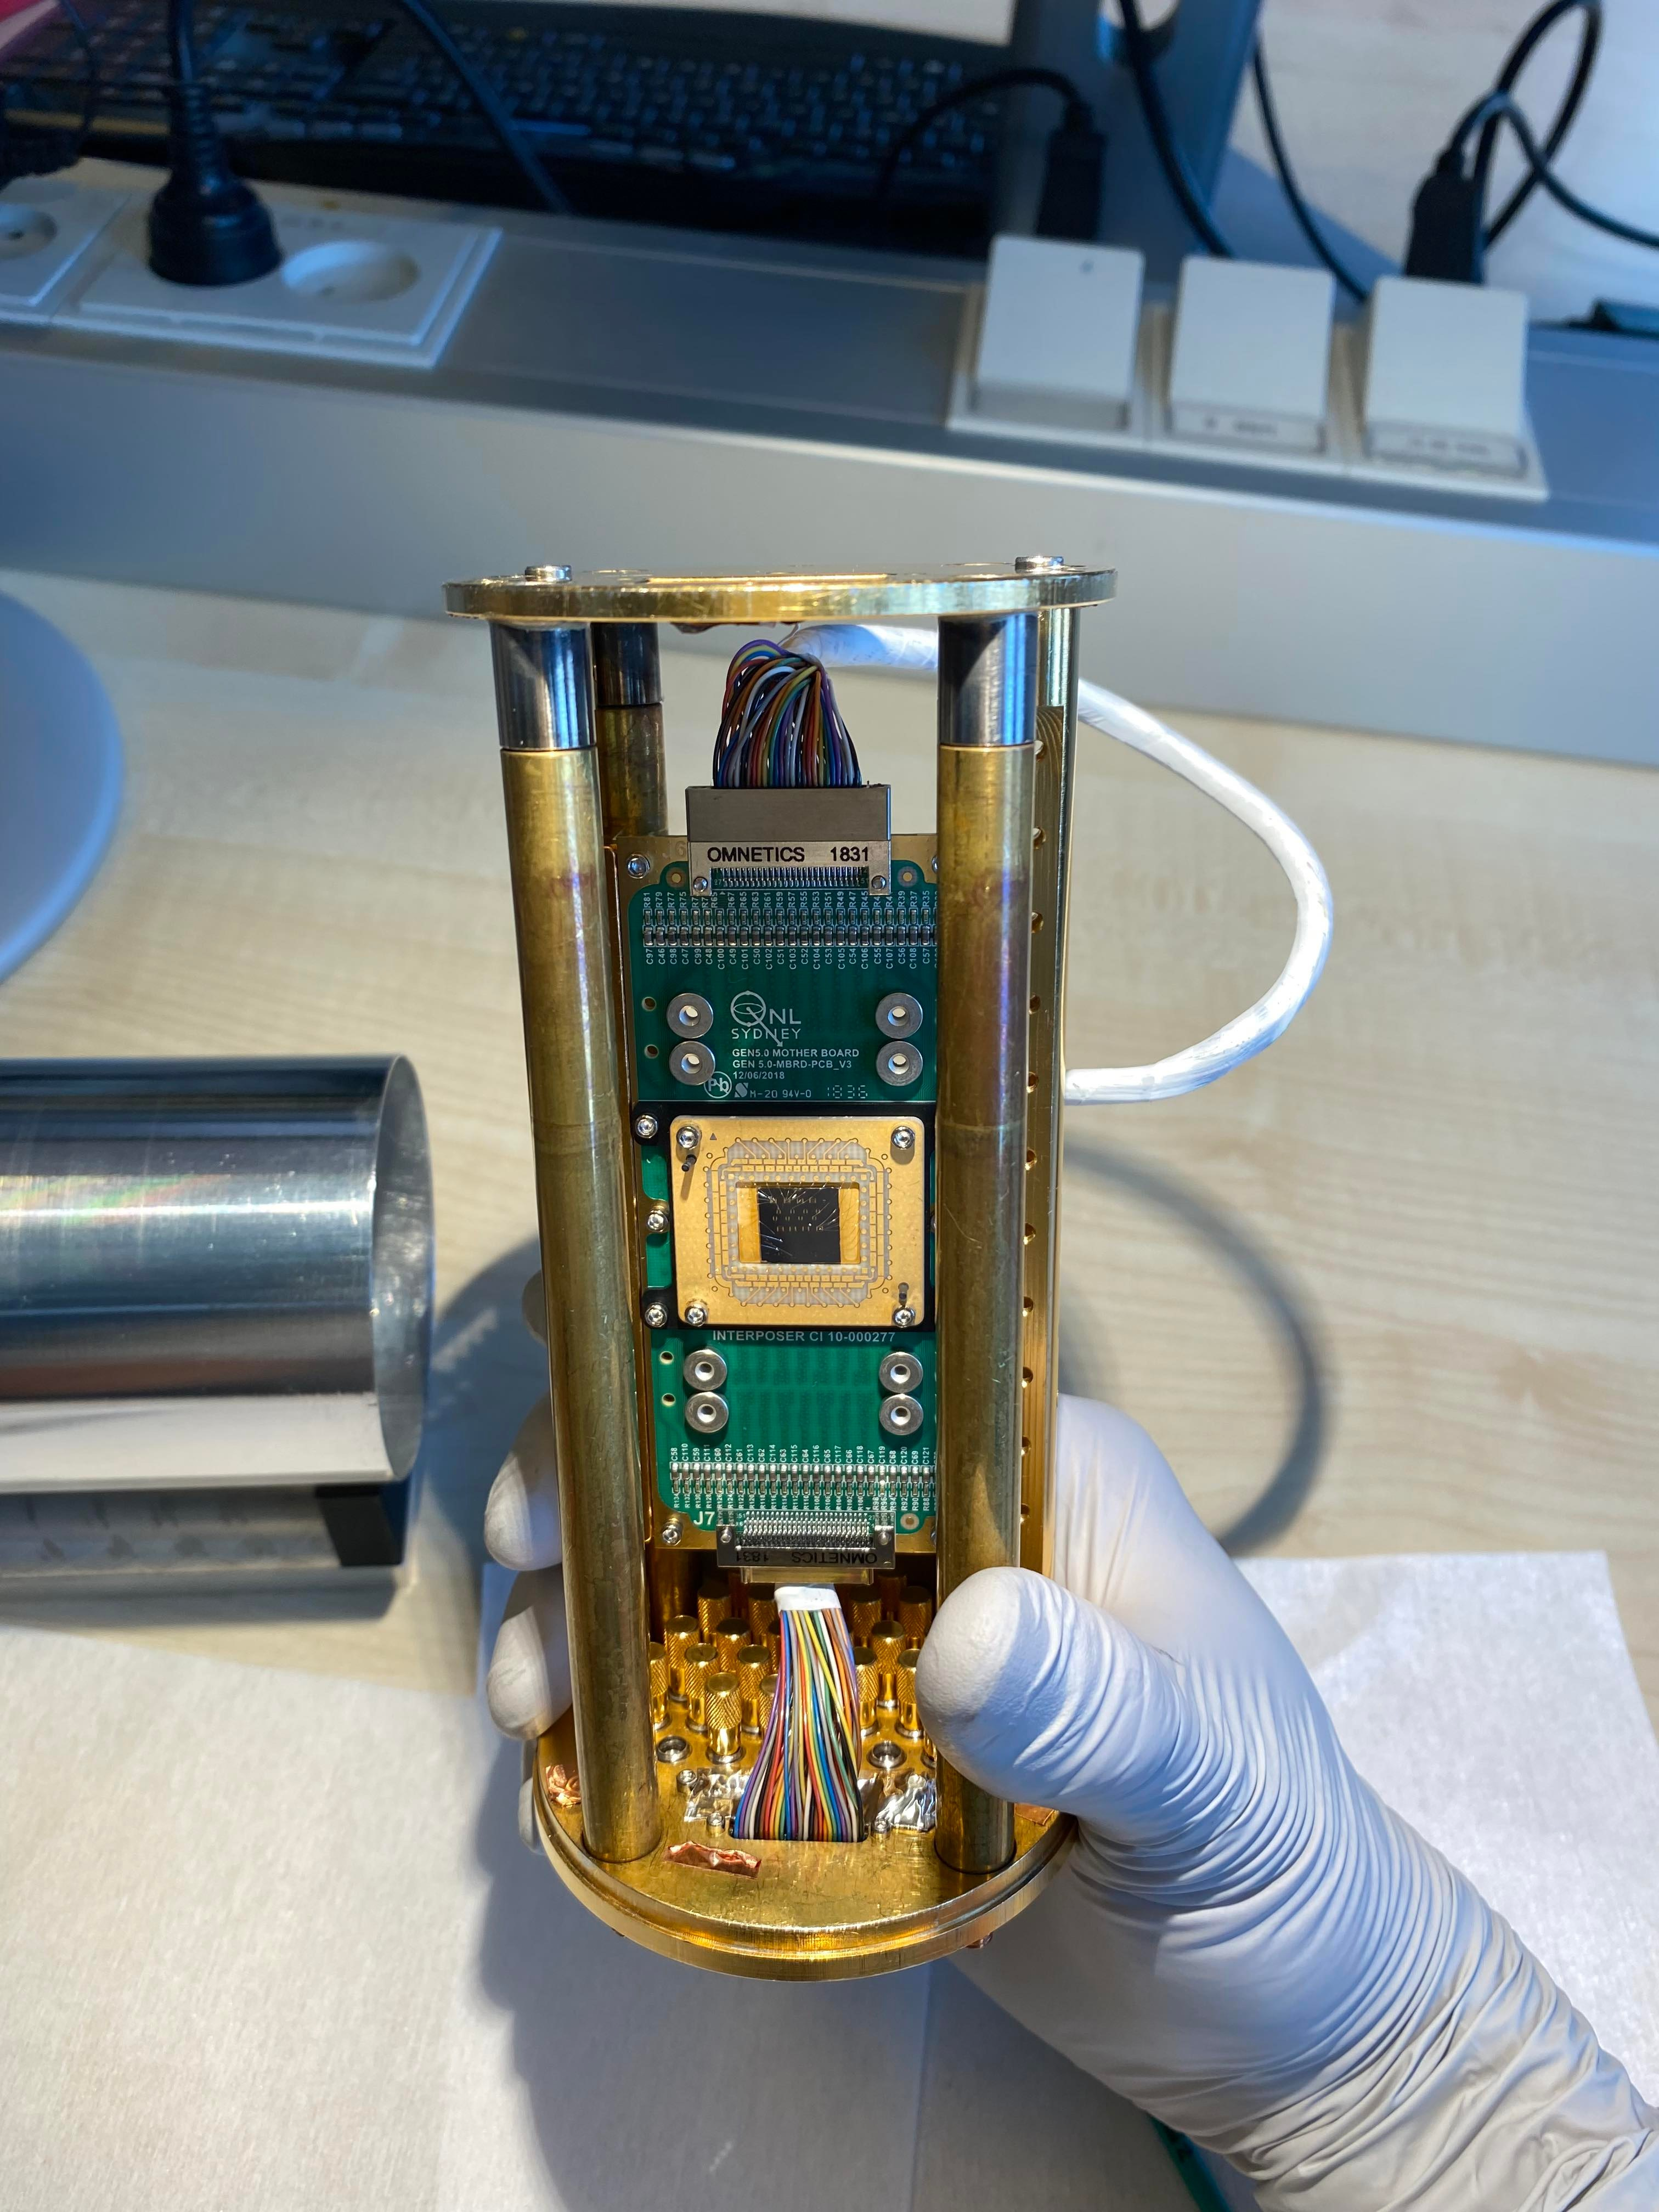
\includegraphics[width=\textwidth]{Pic/PuckSydneyboard.jpg}
         \caption{}
         \label{}
     \end{subfigure}
     \hfill
     \begin{subfigure}[b]{0.45\textwidth}
         \centering
         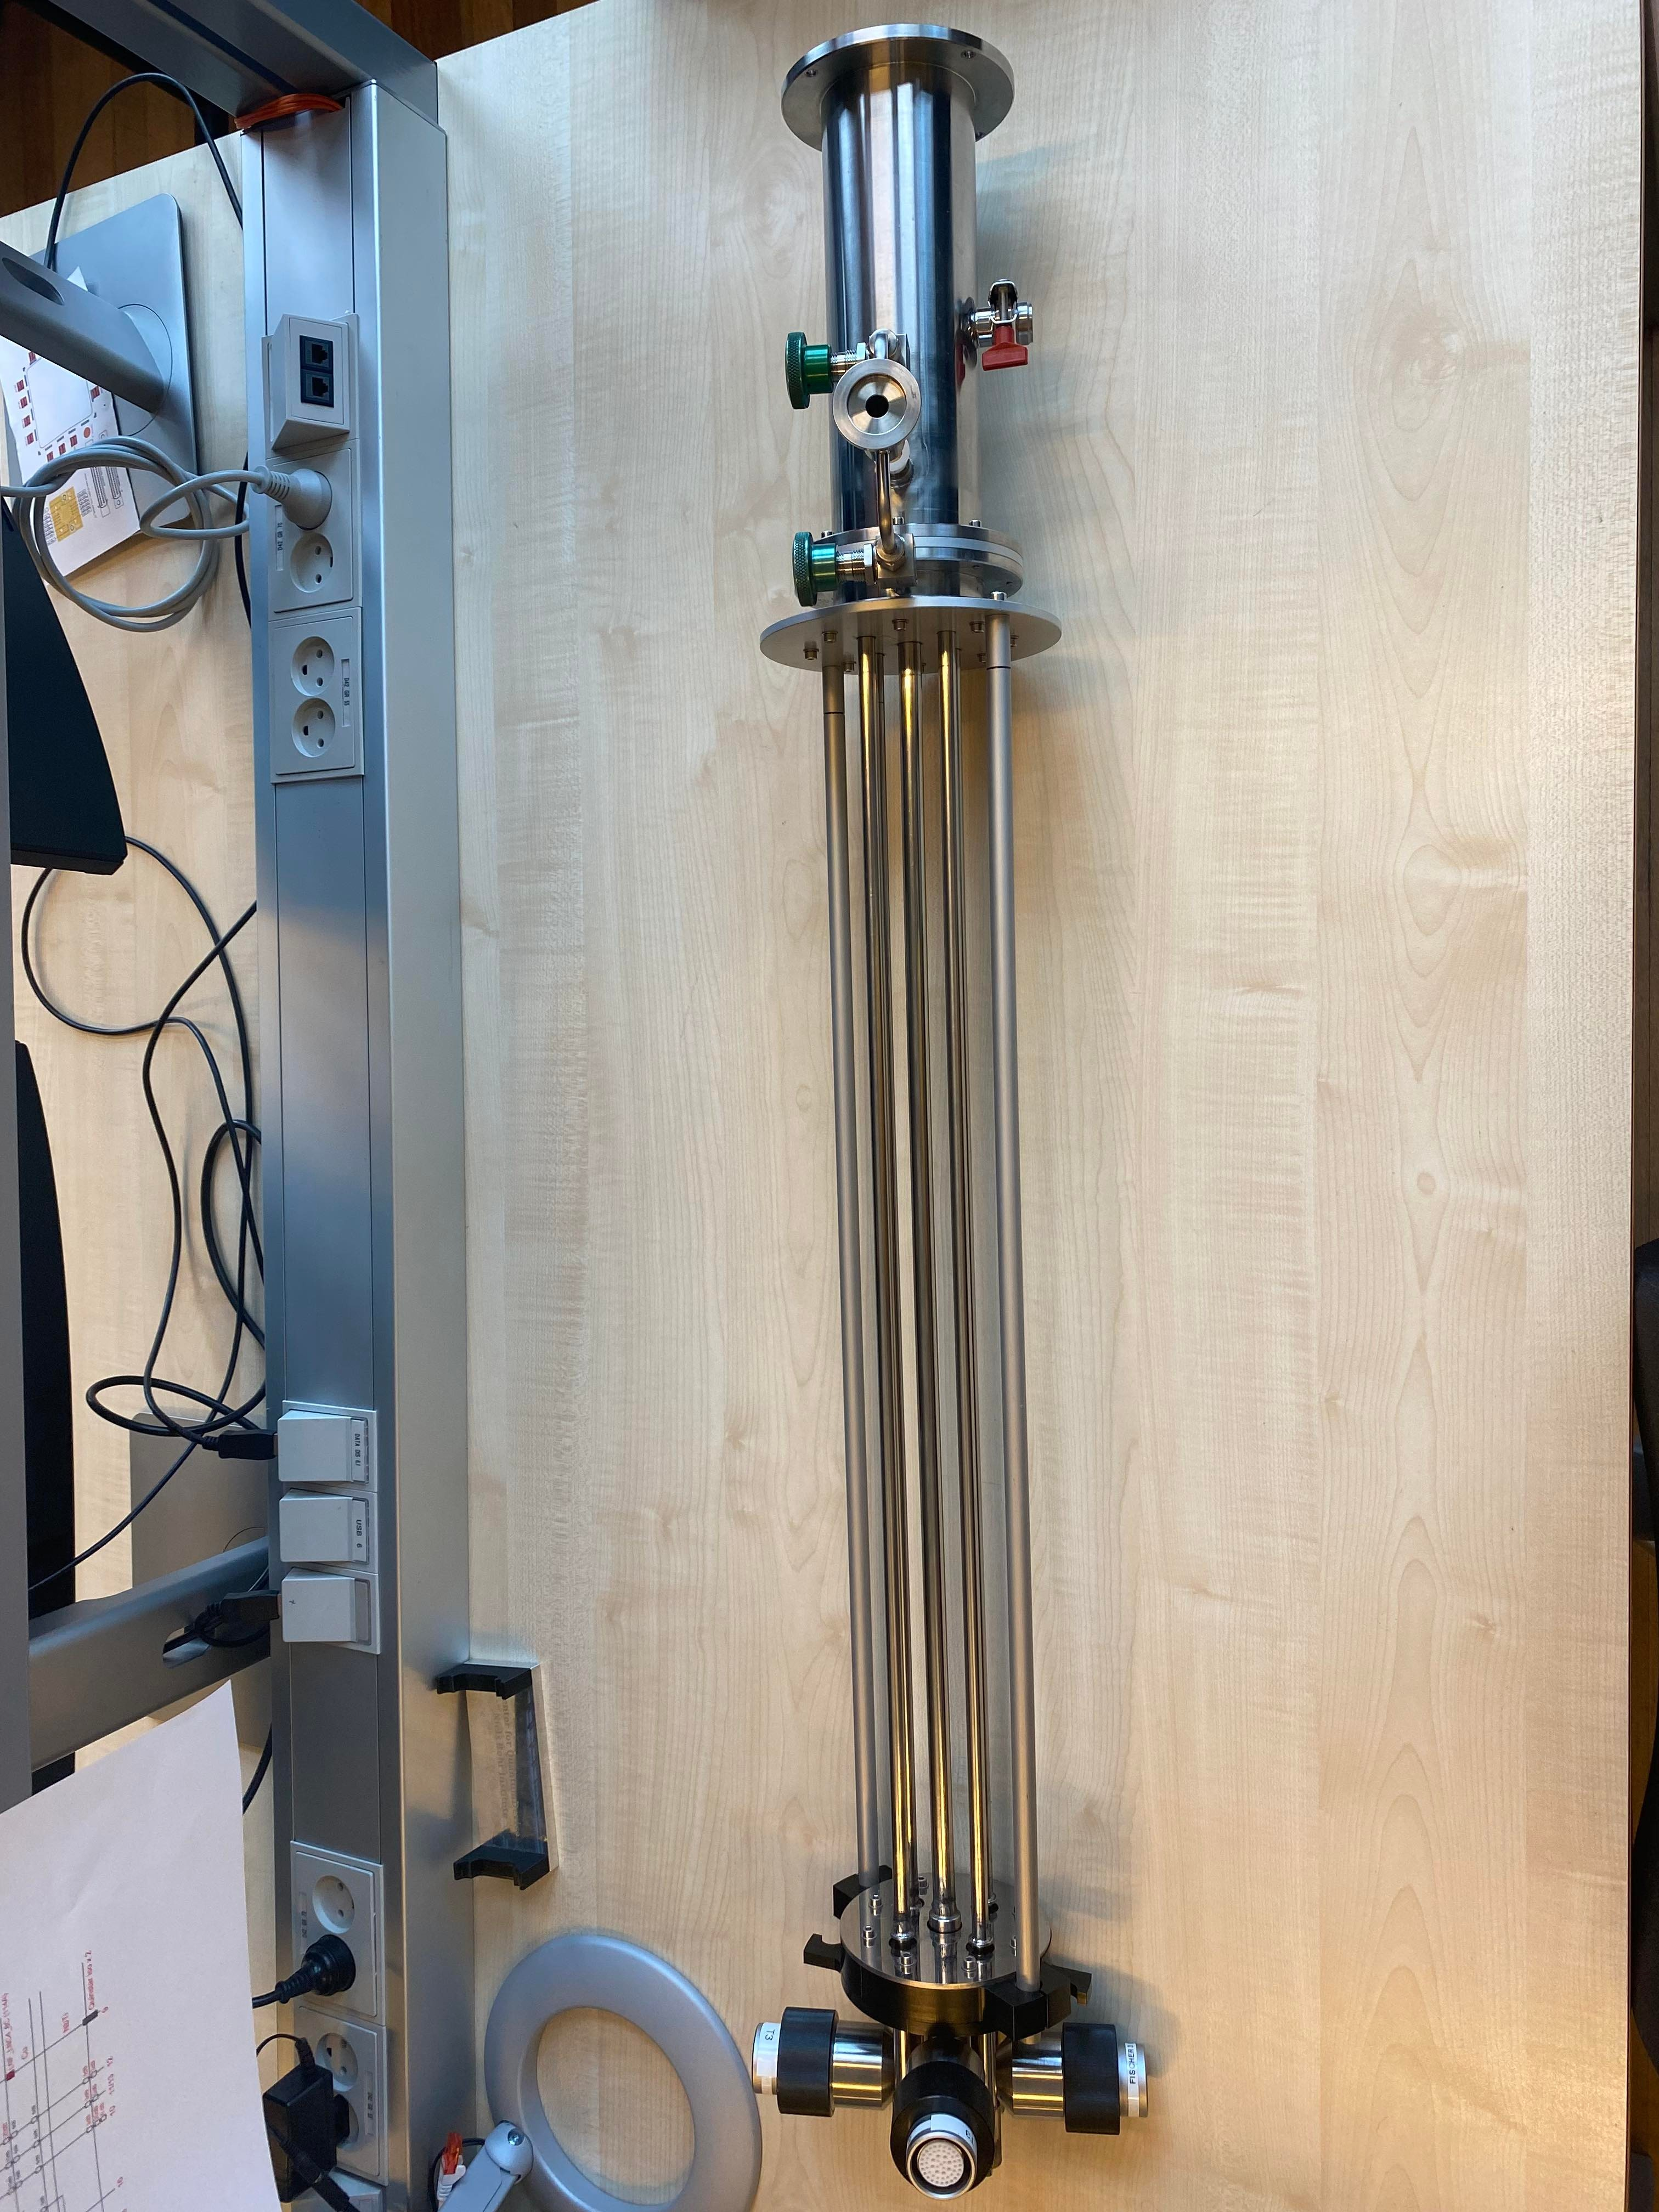
\includegraphics[width=\textwidth]{Pic/Loadrod_2.jpg}
         \caption{}
         \label{}
     \end{subfigure}
    \caption{(a) The puck with Copenhagen board v8p0 on and a nano-D wire connected. (b) The loading rod is hanging on the arm.}
    \label{}
\end{figure}

We need to assemble the motherboard with the puck through 4 rods to load in the sample. Grounding yourself is required during the assembly process. Then we use a loading rod to push them together into the fridge. Grounding the rod during loading is also essential to protect TWPA and nanowires.

\subsection{DC transport measurement setup}
\begin{figure}[h!]
    \centering
    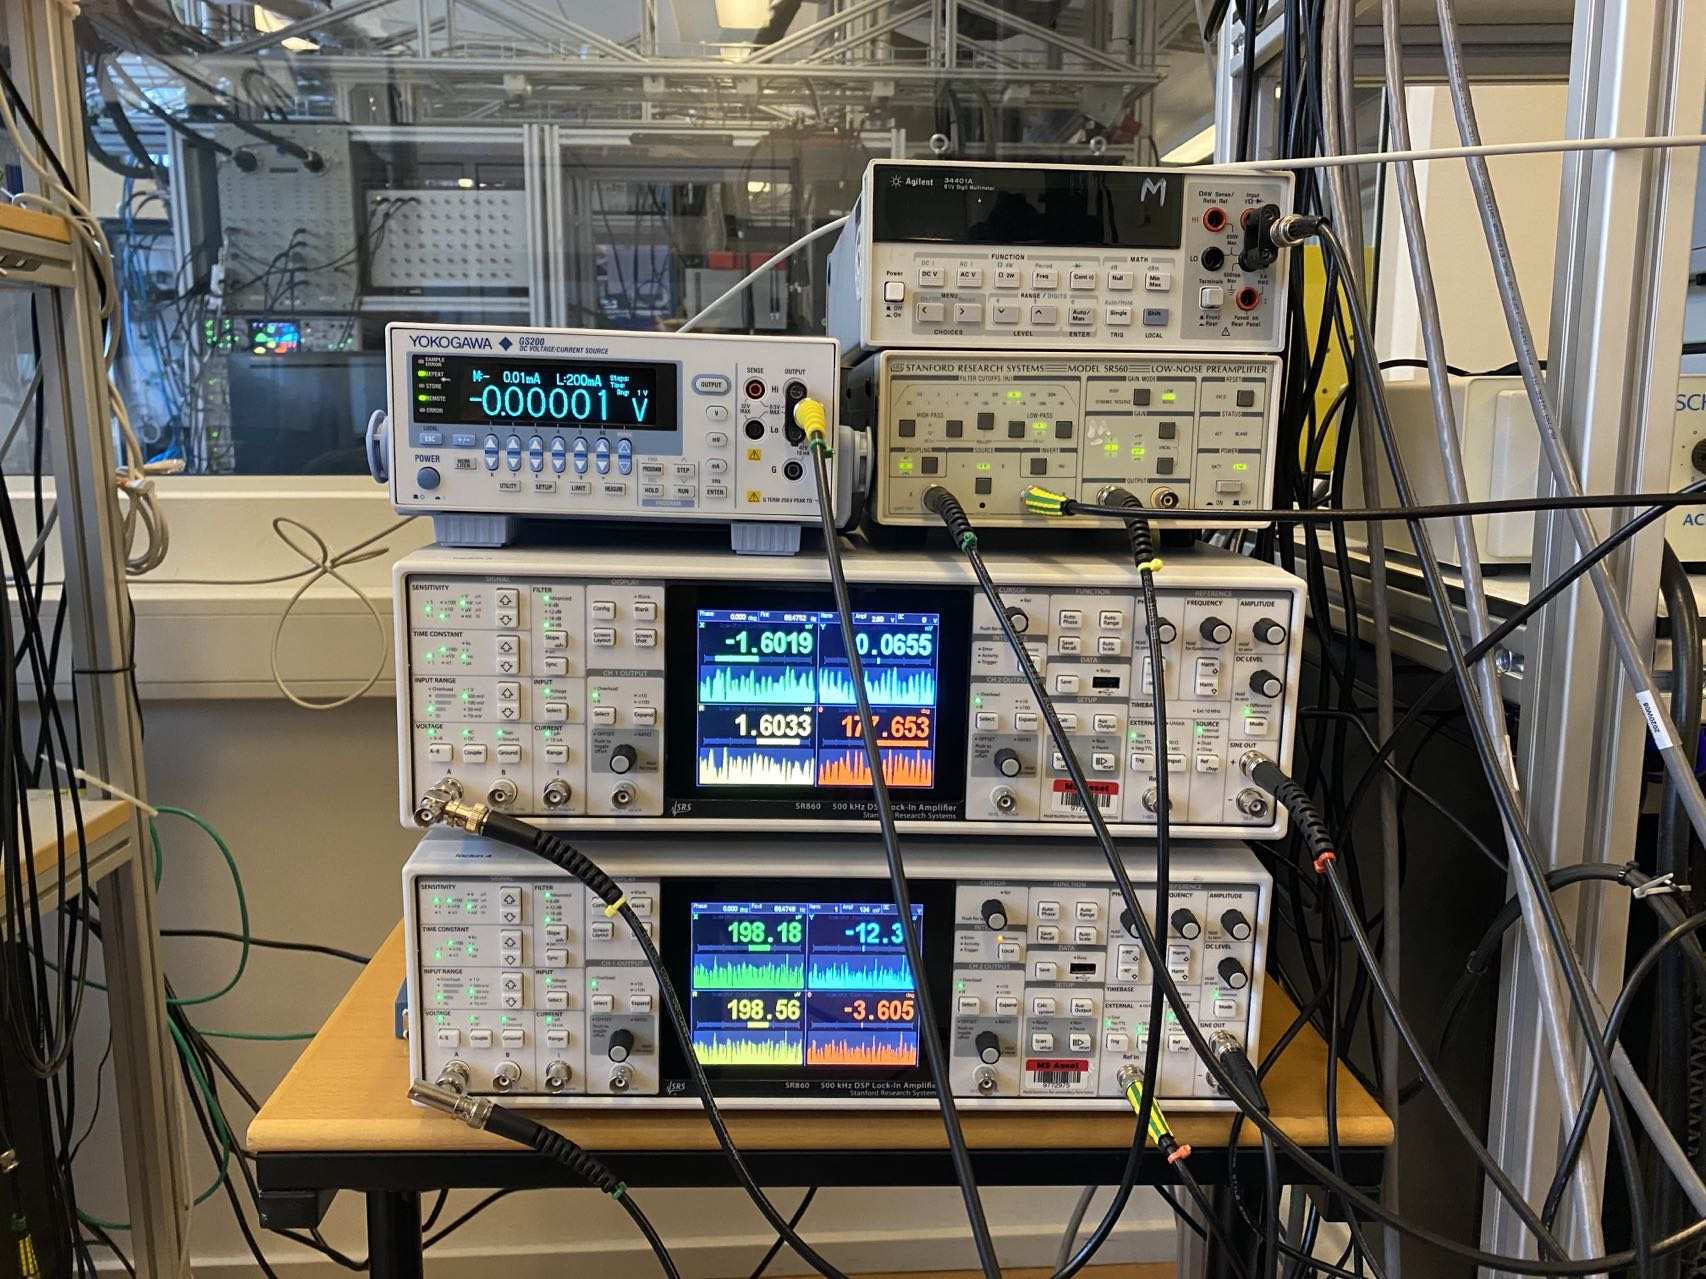
\includegraphics[scale=0.2]{Pic/DCmsmt.jpg}
    \caption{The picture contains two SR865 Lock-in amplifiers (bottom two), one YOKOGAWA as voltage source (upper left), one SR830 as a differential voltage amplifier, and one digital multimeter (DMM, the upper right one). All the low frequency (f <100 Hz) and DC signals are linked to the breakout box through low noise BNC cable. The Keithley 2600 (not shown) is used to apply gate voltage.}
    \label{DCmsmt}
\end{figure}
With four bonds directly on the capacitor pads, we can do four-terminal measurements on the nanowires. There are two types of cryogenic environments to do the transportation measurement, the board station with a base temperature of 5 K and a dilution fridge, but the measurement circuit is the same. We here use the double lock-ins technique, a high accuracy ac signal to do the measurement. Lock-in amplifiers use phase-sensitive detection\cite{RN42} to single out the specific frequency we set and reject the other noisy signals in different frequencies. The output AC signal can describe as the mixture of reference and measurement signal of lock-in:
\begin{equation}
\begin{array}{cc}
         V_{psd} &= V_{sig}V_L\sin(\omega_{sig}t+\theta_{sig})\sin(\omega_L t +\theta_{ref})  \\
     & = \frac{1}{2}V_{sig}V_L\cos{([\omega_{sig}-\omega_L]t+\theta_{sig} - \theta_{ref})} \\
     &-\frac{1}{2}V_{sig}V_L\cos{([\omega_{sig}+\omega_L]t+\theta_{sig} + \theta_{ref})}
\end{array}
\end{equation}
where $V_{sig}$ is the output voltage from the measurement circuit, $V_L$ is the lock-in amplifier's internal reference signal voltage. While $\omega_{sig} = \omega_L$, we will see that the difference frequency term is what we need as a very nice DC signal. The frequency is usually set as a prime number far from 50 or 100 Hz, such as 17.177Hz.
\begin{figure}[h!]
    \centering
    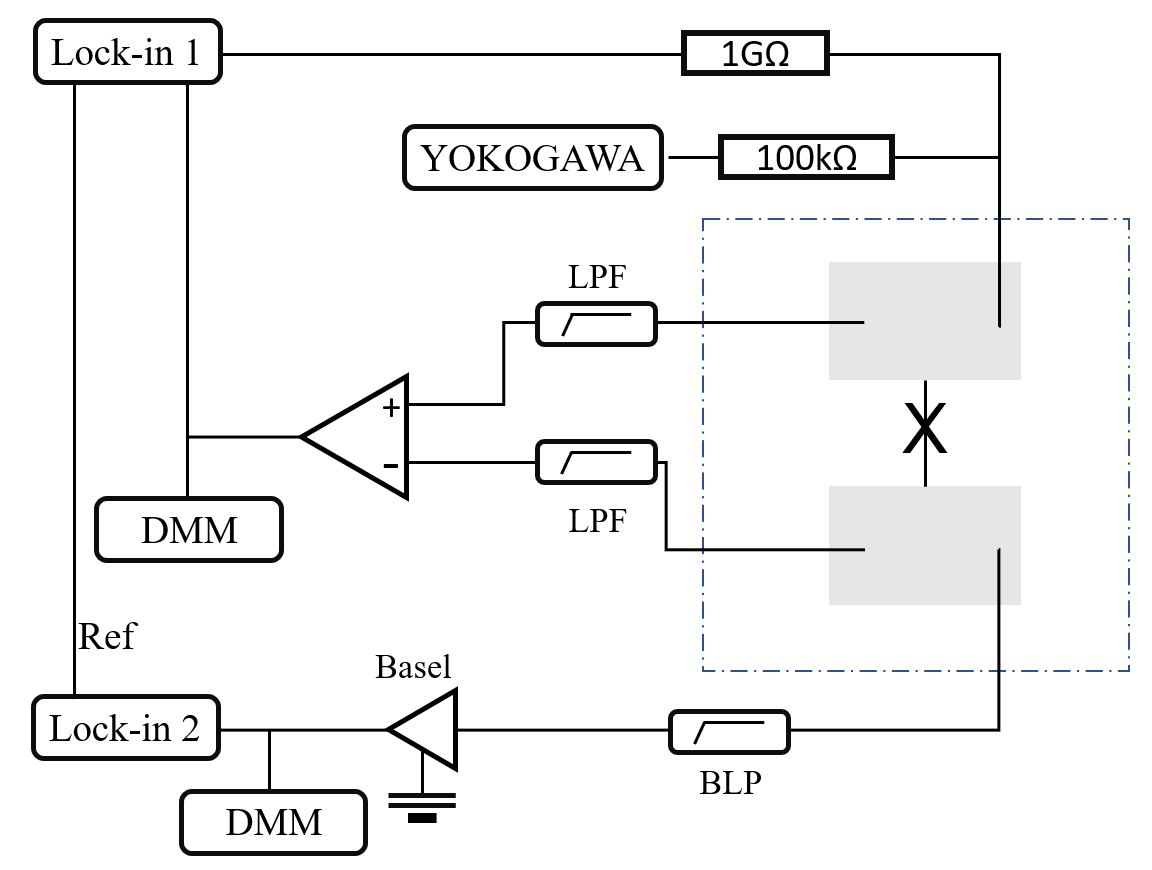
\includegraphics[width=0.65\linewidth]{Pic/Ibias_circuit.png}
    \caption{The two lock-ins' current bias measurement circuit. We use Lock-in amplifiers, SR830 or SR865 from Stanford Research System, as AC signal detectors. YOKOGAWA GS200 serves as a DC voltage bias source, then converts to current bias through the resistor. DMM is a digital multi meter as the monitor for gross voltage signal. Basel is the current-voltage converter, which turns the current signal to voltage and amplifies it. BLP and LPF are both low-pass filters. }
    \label{IbiasDCmsmt}
\end{figure}
\begin{figure}[h!]
    \centering
    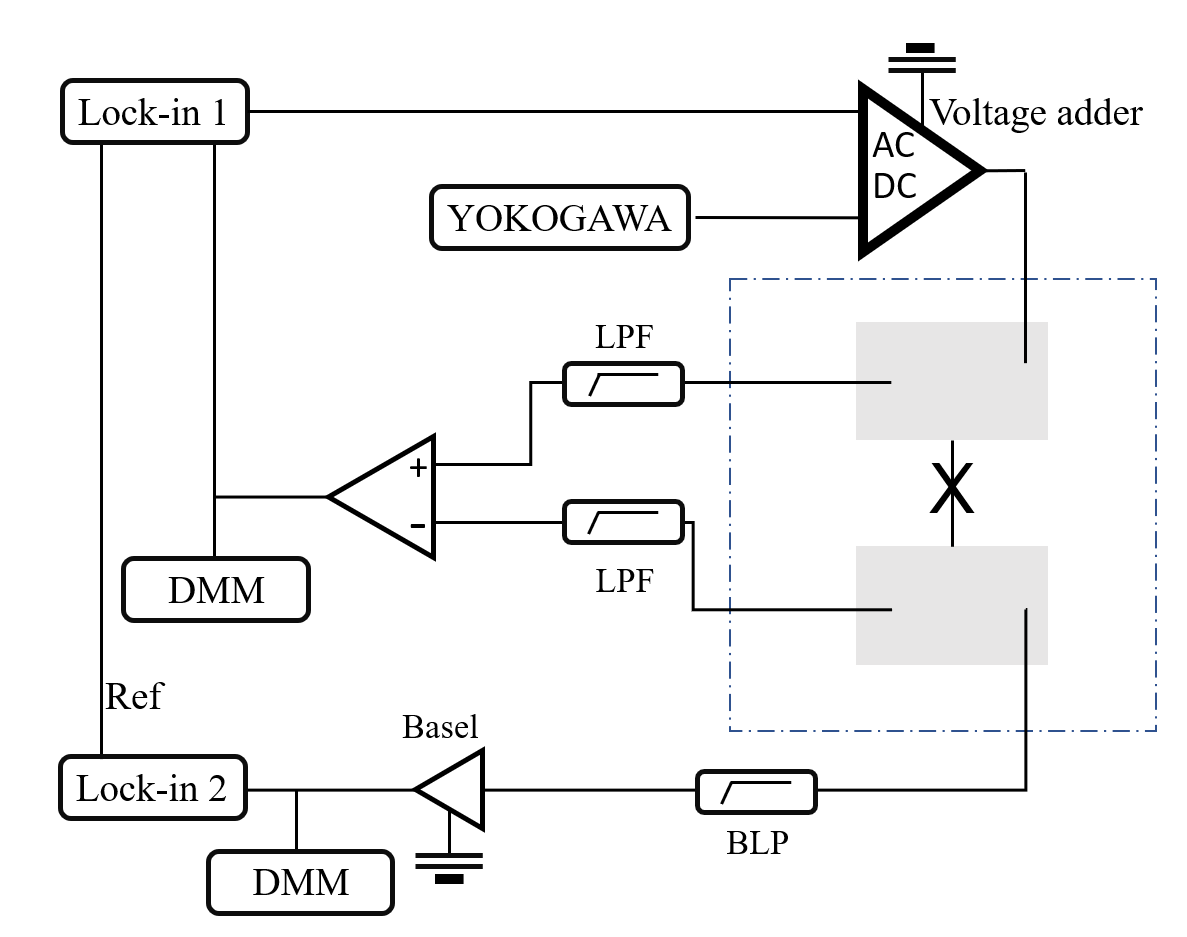
\includegraphics[width=0.65\linewidth]{Pic/Vbias_circuit.png}
    \caption{The voltage bias measurement is the similar configuration as the current bias measurement, but replace the resistors with a voltage adder.}
    \label{VbiasDCmsmt}
\end{figure}
There are two measurement types, current bias (I bias) and voltage bias (Vbias). The current bias is used when the junction is in the metallic regime to measure the critical current of the qubit system (including bulk aluminum or tantalum). We usually set the AC current to 1nA (corresponding to 1V output from Lock-in on 1G$\Omega$ resistor) and apply bias current up to 30nA. As the gate voltage tunes down, the normal resistance of the nanowire goes up and approaches over $10^{7}\Omega$ magnitude. We define this regime as the tunneling regime. The I bias measurement is risky now because the voltage output voltage from YOKOGAWA and lock-in is mostly applied on nanowires and thus potentially blows them up. Vbias measurement in this regime is used to precisely control the voltage applied to the nanowires. We use a voltage adder, which combines the AC and DC voltage and outputs an attenuated voltage. Meanwhile, we can observe different properties like the superconducting gap of the system, MAR. 
\begin{figure}
    \centering
    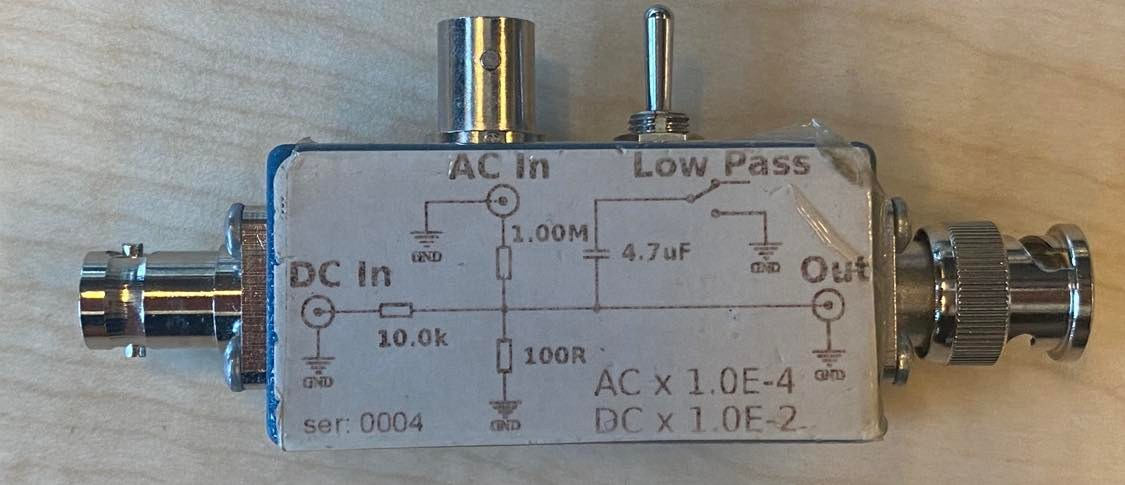
\includegraphics[width=0.6\textwidth]{Pic/Voltageadder.jpg}
    \caption{The voltage adder we are using for voltage bias measurement.}
    \label{fig:my_label}
\end{figure}
The output AC bias voltage on the nanowire is now around 10 $\mu eV$ (which is 100 mV output from the Lock-in). The voltage bias measurement is only used in the dilution fridge since the nanowire and the bulk aluminum, tantalum, are both not becoming superconducting in the board station (the base temperature at around 5 K).

\subsection{High frequency spectroscopy measurement setup}
The high-frequency measurement comes after we understand the transportation property, such as the nanowires' critical current and superconducting gap. The measurement is done in the dilution fridge. We use two types of setups, one is the vector network analyzer (VNA) in frequency domain measurement to find the resonance peak for readout and qubit manipulation frequency, and the ALAZAR digitizer in both frequency and time domain measurement.

\subsubsection{Resonator spectroscopy}
VNA is a powerful tool to sweep a wide range of frequencies and return a $\mathbf{S}$-parameter matrix. Experimentally, we mainly focus on S21 since it tells us the transmission signal through the device under test (DUT). When a mutually or capacitively coupled resonator is in resonance with the input signal, we will clearly see a dip in the S21 signal. Usually, we will sweep the frequency in high power, for example, 0 dB output on VNA and -80dB on line attenuation, to spot the bare cavity resonance frequency. We then do a power sweep on the TWPA to find the best pump power with a high signal-noise ratio (SNR). After that, we do a power sweep on the resonator and find the lowest power with a visible resonator shape. More details are at \textbf{Chapter 6} 

% \subsubsection{Two-tone spectroscopy}
% While the resonator is coupled to a qubit, and we can see punchout effect when the RF output is in low readout power (lower than the critical photon number $n_c$ of the resontor), meaning the single resonant mode in the cavity is not saturated. This is an important sign of the presence of a qubit. In the case of transmon with dispersive readout, we can know the rough region by the direction of punchout from high to low readout power. If the qubit frequency is lower than resonator frequency, the punchout will be to the right. vise versa.

% After that, we go for the two-tone spectroscopy, which shows the spectrum by driving the resonator and the qubit. Now we need the aid of RF generator to continuously drive the resonator, and use VNA to sweep on the drive line or transmission line. When the frequency hits on 0-1 transition frequency $f_{01} = \omega_{01}/2\pi$, there exist a dip on the qubit spectroscopy. As driving in a higher power, we can even see $\f_{02}/2$ and sometimes $\f_{03}/3$, that further confirm the existence of a qubit. 

% The next step is to optimize the readout frequency. As Eq showing, different state of transmon will lead to diverse readout frequency. If the detuning between the resonator frequency and qubit frequency $\Delta_0 = \omega_r - \omega_{01}$ versus qubit frequency $\Delta_0/\omega_{01}$ is large enough, the resonator frequency will shift left while qubit is excited. Therefore, we can set the readout frequency between the two resonator state to get a better SNR. 
